\documentclass[a4paper,12pt, final]{report}
\usepackage{graphicx}
\usepackage{caption}
\usepackage[T1]{fontenc}
\usepackage{listings}
% \usepackage{url}
% \PassOptionsToPackage{hyphens}{url}\usepackage{hyperref}
\usepackage{xurl}
\usepackage{multirow}
\usepackage{float}
\usepackage{mdframed}
%\usepackage[nomain,acronym,xindy,toc]{glossaries} % nomain, if you define glossaries in a file, and you use \include{INP-00-glossary}
%\makeglossaries
%\usepackage[xindy]{imakeidx}
%\makeindex
%\usepackage[section]{placeins}
\renewcommand\bibname{References}
\usepackage[utf8]{inputenc}
%\usepackage{algorithm2e}
%\usepackage{wrapfig}
\usepackage{epsfig}
%\usepackage{hyperref}
\usepackage[hidelinks]{hyperref} % To Hide the box around links
\hypersetup{
    colorlinks=true,
    linkcolor=blue,
    filecolor=magenta,      
    urlcolor=blue,
    pdftitle={Overleaf Example},
    pdfpagemode=FullScreen,
    }
\urlstyle{same}
\renewcommand\bibname{References}
%\usepackage{algorithm2e}
\usepackage{color}
\usepackage{textcomp}
\usepackage{acronym}
\usepackage[top=0.5in, bottom=1in, left=1in, right=1in]{geometry}

% for sorting the references appearance-based
\usepackage[sorting=none, style=ieee]{biblatex} 
\bibliography{main}

\usepackage{xcolor}
\definecolor{dark-red}{rgb}{0.4,0.15,0.15}
\definecolor{dark-blue}{rgb}{0.15,0.15,0.4}
\definecolor{medium-blue}{rgb}{0,0,0.5}

% colors for code listing
\definecolor{codegreen}{rgb}{0,0.6,0}
\definecolor{codegray}{rgb}{0.5,0.5,0.5}
\definecolor{codepurple}{rgb}{0.58,0,0.82}
\definecolor{backcolour}{rgb}{0.95,0.95,0.92}

\lstdefinestyle{mystyle}{
    backgroundcolor=\color{backcolour},   
    commentstyle=\color{codegreen},
    keywordstyle=\color{magenta},
    numberstyle=\tiny\color{codegray},
    stringstyle=\color{codepurple},
    basicstyle=\ttfamily\footnotesize,
    breakatwhitespace=false,         
    breaklines=true,                 
    captionpos=b,                    
    keepspaces=true,                 
    numbers=left,                    
    numbersep=5pt,                  
    showspaces=false,                
    showstringspaces=false,
    showtabs=false,                  
    tabsize=2
}
\lstset{style=mystyle}

\newcommand{\BigO}[1]{\ensuremath{\operatorname{O}\bigl(#1\bigr)}}
\parindent 8pt
\begin{document}
    \thispagestyle{empty}
    \vspace*{1cm}
{
    \centering
    \textbf{\LARGE Performance characterization of GPU-based\vspace{10pt}\\
    VDI and virtualized graphics acceleration}\\
    \vspace{1.20cm}
    %\it
    %\vspace{.5cm}
    %\rm
    \textbf{\large RnD Report - Spring 2023-24}\\
    \vspace{1cm}
    \large{\textbf{CS 490}}\\
    \large{\textbf{RnD Project I}}\\
    \vspace{1.50cm}
    {by}\\
    \vspace{0.20cm}
    \textbf{\large Anshika Raman}\\
    \vspace{0.25cm}
    \textbf{\large (Roll No. 210050014)}\\
    \vspace{1.8cm}
    {Under the guidance of}\\
    \vspace{0.20cm}
    \textbf{\large Prof. Purushottam Kulkarni}\\
    \textbf{\large Prof. Parag Chaudhuri}\\
    \vspace{0.30cm}
    \vspace{1.450cm}
    
    \begin{figure}[htb]
        \begin{center}
\includegraphics[height=1.5in,width=1.5in]{images/iitblogo.png}
        \end{center}
    \end{figure}

    {\textbf{Department of Computer Science and Engineering}}\\
    {\textbf{Indian Institute of Technology Bombay}}\\[10pt]
    {\textbf{April 2024}}
    
}

\renewcommand{\abstractname}{\large Acknowledgement}
\begin{abstract}
    I express my gratitude to my guide, Prof. Purushottam Kulkarni, and my co-guide, Prof. Parag Chaudhuri, for providing me with the opportunity to work on this topic. 
    \\\\
    \\\\
    \\\\
    Anshika Raman\\
    Computer Science and Engineering\\
    IIT Bombay\\\
\end{abstract}

\clearpage

\renewcommand{\abstractname}{\large Abstract}
\abstract{Virtual Desktop Infrastructure (VDI) makes a remote desktop machine available on the go or, in other words, accessible from anywhere. It eliminates the need for having a dedicated physical machine for each individual in an organization and the need for installing and updating apps on individual machines since virtual desktops are centrally managed. Also, the endpoint devices can be less powerful since most computing happens in the data centre. The benefits of VDI are improved performance, security, lower hardware requirements, scalability, and cost savings, and it also enables BYOD (bring your own device). With VDI, instead of running the OS and apps on the hardware, it runs on a VM hosted by the hypervisor. Previously, only one user could access a virtual desktop from a single OS. However, the VDI allows many users to share an OS running on multiple desktops. With its evolution, VDI is no longer constrained to low-resolution desktops but can now deliver high-resolution, 3D desktops to many users. VDI offers different workloads, ranging from 3D desktops to high-performance 3D applications like AutoCAD. End users of such a setup expect reliable and consistent performance, and a slowdown will indicate an overburdened CPU. Thus, the tasks of desktop rendering in the case of VDI should be off-loaded from the CPU to the GPU for better performance and to let the CPU focus on other essential processes. Hence, we require a hardware-accelerated VDI setup or VDI that can utilize the GPU to improve the performance.\\

\noindent VDI is generally set up in a data centre or a server, and it hosts virtual desktops through virtual machines. Multiple users connect to the VDI server to access their individual desktops remotely from an endpoint device. To support such parallelism in desktop rendering, the GPU(s) available at the server are multiplexed. GPU(s) are virtualized to provide this support inside the VMs; in other words, a shadow of the server GPU(s) is created for use by VMs. GPU Virtualization models like hardware-assisted (multiple GPU instances or slices of physical GPU are created, one for each VM), pass-through (physical GPU is completely allocated only to one of the VMs), and paravirtualized (a fake or virtual GPU without additional hardware support is made available per VM) can be employed to introduce virtual GPUs within VMs. The performance of these models decreases in the order of hardware-assisted, pass-through and paravirtualized.\\

\noindent Now, the hardware-accelerated VDI is not readily available as free for use. Few platforms like NoMachine allow leveraging \verb|nvenc| encoder of Nvidia GPUs to encode frames for VNC display. However, this service is unavailable for multiple clients in the non-proprietary (unpaid) version. Hence, this RnD work aims to design a setup capable of providing multiple isolated hardware-accelerated desktops for clients via VNC, with a hypervisor running on the host machine. Through this work, we demonstrate such a setup, the design choices of various tools, and finally evaluate the setup's performance.}

\tableofcontents
\addcontentsline{toc}{chapter}{\listfigurename}
\listoffigures

% https://tex.stackexchange.com/questions/14510/how-to-show-listoffigures-and-listoftables-on-one-page-and-in-the-toc
\begingroup
\let\clearpage\relax
\listoftables
\endgroup
% \printglossaries

% Chapter 1
\chapter{Introduction}

The days when one needs to be present in the office to access your data/desktop is the story of the past. With VDI, one can access their cloud desktop from anywhere. This RnD work discusses the benefits and prospects of software with hardware-accelerated VDI, which provides organizations with new opportunities to enhance their efficiency and create new growth points. Today, the business environment is characterized by constant changes, and the requirements for flexibility and scalability of the computing infrastructure are growing. VDI is the concept implemented in organizations to provide essential resources for remote work and create the best control conditions. It is worth noting that software implementations with the best hardware acceleration perform many graphic processing tasks, making it possible for companies to scale their activities seamlessly.\\

\noindent Typically, the VDI is set up on a server machine that hosts multiple desktops within VMs. Users utilizing the VDI service can run various compute-intensive workloads like 3D applications, such as AutoCAD, Blender, etc. At the server end, these computations can be quite heavy, especially when multiple VMs are hosted on a single server. To provide reliable and consistent performance, the desktop rendering tasks are shifted from the CPU to the GPU(s) available on the server machine. Hardware-accelerated VDI setup thus boosts performance.\\

\noindent A variety of possible mechanisms and configurations, like GPU multiplexing, the workload split between GPU and CPU, network bandwidth, etc., can easily influence such a VDI setup. The scope of this work is to draw a correlation between these factors and their influence on performance and cost (CPU, GPU usage, etc.).\\

\noindent Below are the questions pertaining to hardware-accelerated VDI setup this work attempts to answer:
\begin{itemize}
    \item What are the popular VDI services, and why did we choose one over the other?
    \item Why a VM-based setup is necessary, and why should the VMs be hardware-accelerated for rendering desktops?
    \item What is the need for doing performance characterization of VDI setup, and why is the performance-cost tradeoff of hardware-accelerated VMs required to be determined?
\end{itemize}

\newpage

\noindent Let's begin by looking at the advantages and disadvantages of VDI.\\

\noindent \textbf{Advantages}
\begin{itemize}
    \item User has access to data from anywhere.
    \item Accessing the VDI machine does not depend on the specific endpoint, i.e. BYOD (bring your own device).
    \item One can manage all the devices remotely from anywhere instead of managing each device physically to update/ troubleshoot, etc., with local desktops.
    \item Highly scalable, as the IT team can deploy new virtual desktops within minutes.
\end{itemize}

\noindent \textbf{Disadvantages}
\begin{itemize}
    \item The deployment costs are high, both in terms of technologies and human resources.
    \item Access to VDI entirely depends on the network. Either to access it or to provide a good user experience, there needs to be a good and stable Internet connection.
    \item Running resource-intensive applications such as graphic or video conference tools can generate latency, impacting the user experience.
\end{itemize}\\

\noindent \textbf{How does VDI work?}\\

\noindent In VDI, a hypervisor segments servers into virtual machines that host virtual desktops, which users access remotely from their endpoint devices. All the processing of user applications is done on the host server.\\

\noindent VDI can be either persistent or non-persistent. Each type offers different benefits:

\begin{itemize}
    \item \textbf{Persistent VDI}: A user connects to the same desktop each time, and users can personalize the desktop for their needs since changes are saved even after the connection is reset. In other words, persistent VDI acts like personal physical desktops.
    \item \textbf{Non-persistent VDI}: Users connect to generic desktops, and no changes are saved; it is usually simpler and cheaper since there is no need to maintain customized desktops between sessions. Hence, non-persistent VDI is often used in organizations with many employees who perform a limited set of repetitive tasks and don't need a customized desktop.
\end{itemize}

\noindent \textbf{How to implement VDI?}\\ 

\noindent This work answers the question in much detail. There are three major aspects that this work explores:

\begin{itemize}
    \item Measuring VDI performance %talks about nomachine
    \item Multiplexing the VDI setup with Graphics Acceleration support %talks about vm setup with vnc
    \item Virtualizing the graphics pipeline for hardware acceleration %talks about hardware acceleration inside vm
\end{itemize}

\newpage

\noindent Following are the sections of this work:

\begin{itemize}
    \item Chapter 2 introduces the VDI model, the popular VDI setups, how they work, and the conclusion of our setup.
    \item Chapter 3 provides a detailed description of Graphics Acceleration, its three major models and the support provided by QEMU/KVM. We also describe the popular GPU performance monitoring tools and evaluate the performance of a graphics-accelerated VM.
    \item Chapter 4 discusses the procedure for setting up a graphics-accelerated VM in detail and the experiments performed to measure the performance and cost metrics.
    \item Chapter 5 highlights the shortcomings of the current work and the scope this work has in future.
\end{itemize}

% Starting from the first principles, what does VNC 
% \section{VNC/VDI} % methods - tiger/turbo/NoMachine/QEMU % our approach to mutli-client
% Virtual Network Computing (VNC) and Virtualized Desktop Environment (VDI) refer to desktop virtualisation technologies that allow users to access and control the desktop environment over a network remotely. There are a few well-known examples of remote desktop software like AnyDesk and TeamViewer. We looked specifically into the case of TurboVNC/TigerVNC and NoMachine.

% \subsection{TurboVNC/TigerVNC}
% %link https://turbovnc.org/pmwiki/uploads/About/tighttoturbo.pdf
% \begin{itemize}
%     \item TigerVNC is an older version of TurboVNC. TurboVNC is an improved version but still lacks hardware acceleration.
%     \item TurboVNC allows multiple clients to control the screen individually with real-time isolation, which means that each client can control their own cursor irrespective of other clients.
%     \item It creates multiple display sessions, one per client connection. The client needs a VNC client like Remmina or VNC Viewer to access the display and machine IP. For example, \texttt{<IP>:0} will connect to display session 0, and \texttt{<IP>:1} will connect to display session 1.
%     \item But there are two major limitations of choosing Turbo/Tiger VNC for VDI:
%     \begin{itemize}
%         \item It is not hardware accelerated. The display is very pixelated.
%         \item The display sessions are not isolated \textbf{simultaneous connections}, which means that, let's say, if client A creates a directory on the desktop, client B can see it.
%     \end{itemize}
% \end{itemize}

% \subsection{NoMachine}
% NoMachine is another software providing VNC services. The plus point with NoMachine is that it provides hardware acceleration for encoding the VNC display, which makes the client experience much smoother. It also provides network statistics. However, the only limitation is that it does not provide multi-client support in its unpaid version. As it uses a single port for the client connection, two clients cannot access the same display session simultaneously because the host is already busy with the port.

% \subsection{Hardware-accelerated VDI}
% What do we mean by the term hardware-accelerated VDI? \\ \\
% VNC, in its most basic form, first encodes the display on the available compute resources (CPU/GPU) and then sends the encoded packets over the network, which are then decoded on the client side. Any change on the display, such as a single mouse click, is a unique frame, so the VNC server needs to keep sending the encoded display packets to the client repeatedly. Since a lot of graphical data needs to be encoded and transmitted, two bottlenecks that can cause a lagging screen and slow response to the client side are:
% \begin{itemize}
%     \item network congestion
%     \item slow encoding
% \end{itemize}
% Hardware-accelerated VDI tackles the second and the major bottleneck responsible for poor VDI performance. In hardware-accelerated VDI, GPUs (Graphics Processing Units) or dedicated video encoding/decoding hardware are utilized to offload the computationally expensive tasks from the CPU, enhancing the VDI performance manifolds. We can claim this just by comparing the performance of TurboVNC and NoMachine. NoMachine uses a dedicated \texttt{nvenc} encoder on Nvidia GPUs, whereas TurboVNC uses only a CPU for display encoding tasks. But what allows users to create applications with GPU support? OpenGL APIs

% \section{OpenGL} % introduce and tell turbo n all did not have support
% OpenGL is an API/graphics library for rendering 2D/3D vector graphics on the GPU. There are other alternatives like DirectX, Vulkan, and Direct3D, but OpenGL has been very widely used by a lot of applications for a long time, as it is free for use and is supported by Nvidia. For checking OpenGL support on your machine, we can run the \texttt{glxgears} command in the terminal as shown in the image below. \texttt{glxgears} can be installed with the command: \texttt{sudo apt install mesa-utils}
% \begin{figure}[H]
%     \centering
%     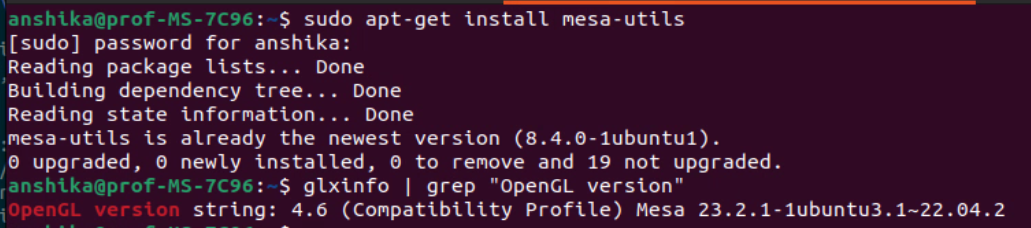
\includegraphics[width=\textwidth]{images/check_opengl.png}
%     \caption{Check for OpenGL support}
%     \label{fig:opengl_verif}
% \end{figure}
% \noindent \textbf{Note:} OpenGL will not work on headless server machines directly. To enable OpenGL rendering on headless server machines, additional software setup such as VirtualGL or a virtual display environment is typically required to provide the necessary graphical context for OpenGL operations. So, we can say that TigerVNC/TurboVNC did not have OpenGL support for graphics rendering. 

% %-------- It is difficult to do GPU passthrough in VirtualBox

% \section{QEMU} % inbuilt vnc, working vm setup, now we need hardware acceleration support inside vm
% %----------explain para/full/hardware accelerated etc
% QEMU is a virtualisation platform that provides built-in support for VNC servers. It is open-source and allows GPU virtualisation. QEMU provides various options for device, display, and networking interface for the VM, which makes it more favourable for experiments. It is lightweight compared to VirtualBox; it doesn't consume much RAM.

% Chapter 2
\chapter{Virtual Desktop Infrastructure (VDI)} %why did we do what we did - like why use all these tools specifically
%check -- make it more like a motivation section

VDIs are key in connecting you with any computer system remotely from any endpoint device, be it your PC, smartphone, tablet, etc. It has played a major role in the IT industry, eliminating the need for the company to provide each employer with a physical machine that needs to be managed, repaired and replaced. Authorized users can access the same company servers, files, apps, and services from any approved device through a secure desktop client or browser.\\

\noindent VDI lets you run traditional desktop workloads on centralized servers and has become the standard. There are multiple ways to deliver virtual desktops and apps to users -- VDI, to be sure, but other flavours of VDI, such as desktop as a service (DaaS) and even personalized Cloud PCs. These services have become increasingly popular for various reasons -- improved security, performance, centralization, lower hardware requirements, and cost savings -- not to mention enabling employees to do their jobs anywhere in the world.

\section{NoMachine VDI}
It is a remote desktop software, free for personal use, designed for anyone who wants to access single or multiple computers using one simple tool. It ensures secure and reliable remote desktop connections, regardless of the underlying network you are using. For personal use (free version), \textbf{only one concurrent} connection is allowed, and hardware-accelerated display processing, video encoding and decoding are also available. \cite{nomachine_intro}\\

\noindent NoMachine allows enabling or disabling the available hardware acceleration for display processing on the server. If the available hardware accelerator is Nvidia GPU, it uses an \verb|nvenc| encoder to encode the display frame buffer.\\

\noindent Since \verb|nvenc| is an efficient encoder w.r.t. time and space, we ran some tests of encoding a 4K video using \verb|ffmpeg| and playing other 4K videos (in a media player like VLC) in parallel, using \textbf{NoMachine VDI}, to provide load on the GPU. To list the available encoders, run the command: \verb|ffmpeg -encoders|. Command to encode a 4K video using \verb|ffmpeg| and \verb|nvenc| encoder:

\begin{mdframed}[backgroundcolor=cyan!20]
    \begin{lstlisting}[language=bash]
ffmpeg -y -vsync 0 -hwaccel cuda -hwaccel_output_format cuda -i input_file.mp4 -c:a copy -c:v h264_nvenc -b:v 5M output_file.mp4
    \end{lstlisting}
\end{mdframed}

\noindent Before running the above command, one must ensure that the Nvidia and the compatible CUDA drivers are installed on the system. We increased the count of \verb|ffmpeg| encoding task and the task of playing 4K video in parallel one at a time.\\

\noindent To monitor the performance of the tests we described, we used the command-line tool \verb|nvidia-smi| to determine the GPU utilization. We observed that for a test where five \verb|ffmpeg| tasks and three video-playing tasks were running parallel, the overall GPU utilization was up to 11\%, but the system RAM (6 GB) and swap memory (2 GB) were being used up. This indicates that our tests did not add enough computational and rendering load on the GPU.\\

\noindent NoMachine also provides its own statistics for a session \cite{nomachine_stats}, which comprises four sections:
\begin{itemize}
    \item NX Cache Statistics: It displays the amount of data cached for each request. A request is a data set travelling from server to client, whereas a reply is a data set travelling from client to server. High cache values indicate an optimized use of bandwidth.
    \item NX Client Side Protocol Statistics: It refers to the data traffic sent from the server to the client.
    \item NX Server Side Protocol Statistics: It refers to the data traffic sent from the client to the server.
    \item NX Protocol Summary: It reports the final and global data on the overall performance.
\end{itemize}

\noindent With these statistics in place, the load on GPU was not observed from the numbers of a NoMachine session. Hence, GPU utilization has no direct correlation with the NoMachine network statistics. Thus, to measure the performance of a VDI server, there needs to be a metric that can compute the GPU performance with the VDI server running.\\

\noindent As the NoMachine statistics did not lead us to some conclusion, we started looking at the close alternatives for a VNC service provider that supports 3D or graphics acceleration, like TurboVNC with VirtualGL support.

\section{TurboVNC + VirtualGL}
TurboVNC is a derivative of VNC (Virtual Network Computing) tuned to provide peak performance for 3D and video workloads. It compresses 3D and video workloads significantly better than the "tightest" compression mode in TightVNC 1.3.x while using only typically 15-20\% of the CPU time of the latter.\\

\noindent All VNC implementations, including TurboVNC, use the RFB (remote framebuffer) protocol to send framebuffer updates from the VNC server to any connected viewers. Each frame buffer update can contain multiple rectangles (regions that have changed since the last update). Each rectangle is then split into multiple subrectangles, and each subrectangle is encoded using the subencoding type that provides the most efficient compression. TurboVNC, when used with VirtualGL, provides a highly performant and robust solution for remotely displaying 3D applications over all types of networks. \cite{turbovnc_intro}

\subsection{VirtualGL}
To display a 3D application running remotely on a cluster, one could use X11 forwarding to display the application on the local machine. This is usually very slow and often unstable.\\

\noindent An alternative approach is to use VNC - also called Remote Desktop - to run GUI applications remotely on the cluster. This approach only works well with applications that only need moderate 3D rendering where software rendering is not good enough. For applications that need to render large complicated models, hardware accelerated 3D rendering must be used.\\

\noindent However, VNC cannot directly utilize the graphic devices on the cluster for rendering. VirtualGL, in conjunction with VNC, provides a commonly used solution for remote 3D rendering with hardware acceleration.\\

\noindent VirtualGL is an open-source toolkit that gives any Linux or Unix remote display software the ability to run OpenGL applications with full hardware acceleration. The OpenGL commands and 3D data are redirected to a GPU in the application server by a technique called \textbf{split rendering}, and only the rendered frames are sent over the network.

\subsubsection{How does VirtualGL accomplish this?}
VirtualGL accomplishes this by pre-loading a dynamic shared object, the VirtualGL Faker, into the OpenGL application at run time. It intercepts and modifies certain GLX, EGL, OpenGL, and X11 function calls to divert OpenGL rendering from the 3D application's windows into corresponding off-screen buffers, which VirtualGL creates in GPU memory on the application server. When the 3D application swaps the OpenGL drawing buffers or flushes the OpenGL command buffer to indicate that it has finished rendering a frame, VirtualGL reads back the rendered frame from the off-screen buffer and transports it.\\

\noindent VirtualGL (VGL) has two built-in image transports that can be used to deliver rendered frames to the 2D X server:

\begin{enumerate}
    \item \textbf{VGL Transport}: It is most often used whenever the 2D X server is located across the network from the application server - for instance, if the 2D X server is running on the client. VirtualGL uses its own protocol on a dedicated TCP socket to send the rendered frames to the client, and VirtualGL Client decodes the frames and composites them into the appropriate X window. It can either deliver the frames in an uncompressed form (RGB-encoded) or compress them in real time using a high-speed JPEG codec.\\
        \begin{figure}[H]
            \centering
            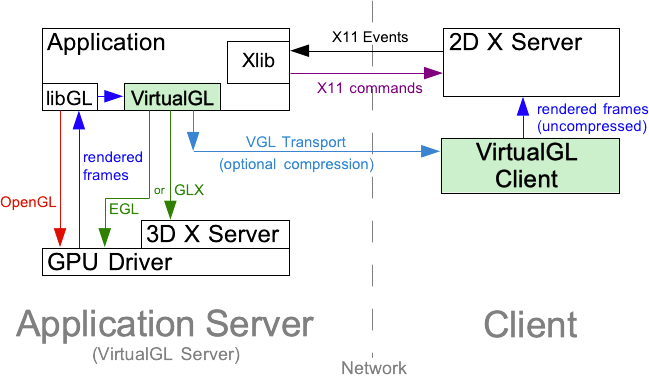
\includegraphics[width=0.8\textwidth]{images/vgltransport.png}
            \caption{VGL Transport with client-side 2D X server \cite{virtualgl_userguide}}
            \label{fig:vgl_transport}
        \end{figure}
    \item \textbf{X11 Transport}: It simply draws the rendered frames into the appropriate X window using \verb|XPutImage()| or similar X11 commands. This is most useful in conjunction with an X proxy. which can be one of any number of Unix remote display apps, such as VNC. In this case, VirtualGL does not normally perform any image compression or encoding itself. Instead, it relies on an X proxy to encode the frames and deliver them to the client(s). Since using an X proxy eliminates the need to send X11 commands over the network, this is the recommended method for using VirtualGL over high-latency or low-bandwidth networks.\\
        \begin{figure}[H]
            \centering
            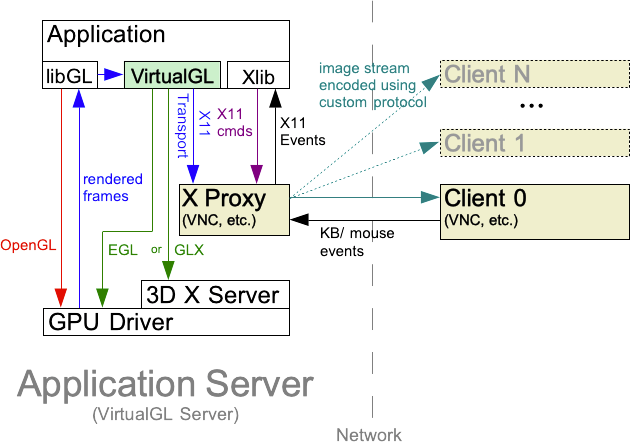
\includegraphics[width=0.8\textwidth]{images/x11transport.png}
            \caption{X11 Transport with an X proxy \cite{virtualgl_userguide}}
            \label{fig:x11_transport}
        \end{figure}
\end{enumerate}

\subsection{Setting up TurboVNC + VirtualGL}
The User Guide of VirtualGL 3.1 \cite{virtualgl_userguide} was followed for configuring a Linux Ubuntu 22.04 LTS machine as a VirtualGL Server, with the GPU of Nvidia GTX9701 (Maxwell architecture).\\

\noindent Although after multiple attempts, by trying the display manager of lightdm instead of the default gdm, the setup did not work, meaning the 3D application process running on the host was not listed within \verb|nvidia-smi|.\\

\noindent One of the possible reasons could be the graphics card. The user guide recommends using a professional-grade GPU such as the \textbf{AMD Radeon Pro} or \textbf{Nvidia Quadro} to set up the VirtualGL Server. We did not have access to such cards and, hence, could not continue with this setup.

% Chapter 3
\chapter{Graphics Acceleration}
%add----write about vm cloning

As described before, the shifting of graphics acceleration hardware from the workstation to a server plays a key role in improving the computing performance for graphics processing. In the VDI setup, the graphics acceleration is made available inside a VM via the virtualization technique. In other words, a shadow of host GPU is introduced in a VM for its own use.\\

\noindent This section describes the methods for GPU virtualization in the use case of VDI and how QEMU supports them. They are as follows:

\begin{enumerate}
    \item Hardware-assisted model
    \item Pass-through model
    \item Paravirtualized model
\end{enumerate}

\section{Hardware-assisted model}
VDI is a great way to deliver remote desktops to users, but it is only viable if those users run apps that do not rely on complex graphics or video rendering. VDI is not ideal for delivering high performance for power users who work with apps that display complex graphics. That's where the \textbf{hardware-assisted} virtualization comes into the picture. This solution adds critical virtualization functions as fast, efficient, new processor commands and has been proven to be a far better approach than software-based virtualization.\\

\noindent This technique is also called as \textbf{mediated pass-through} or \textbf{full GPU} virtualization. The GPU provides contexts and virtual memory ranges for each VM through IOMMU, and the hypervisor sends graphical commands directly to the GPU from guests. This hardware feature allows multiple (virtual) GPUs to be exposed as PCI devices, which can be used via a GPU device driver from within the VM. The GPU-specific extensions at the hypervisor and the hardware-assisted features of the GPU allow multiplexed access to the physical GPU.\\

\noindent Two big GPU vendors, Nvidia and AMD, provide this support on specific professional graphics cards and not consumer cards. Nvidia's technology is called \textbf{vGPU}, while for AMD, it's called \textbf{MxGPU}. \\

\noindent Nvidia has introduced several of these hardware features and corresponding software drivers and a typical hardware-software stack to enable vGPUs-based GPU multiplexing as shown in Figure \ref{fig:nvidia_vgpu_hw_sw_stack}.

\begin{figure}[H]
    \centering
    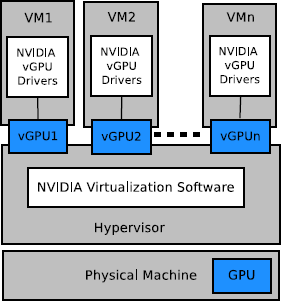
\includegraphics[width=0.4\textwidth]{images/nvidia_vgpu_hw_sw_stack.png}
    \caption{Hardware-software stack of vGPUs \cite{empirical_analysis_hw_assist_virt}}
    \label{fig:nvidia_vgpu_hw_sw_stack}
\end{figure}

\noindent Nvidia vGPU enables multiple VMs to have simultaneous, direct access to a single physical GPU, using the same Nvidia graphics drivers deployed on non-virtualised OS. vGPU software supports GPU instances on GPUs that support the Multi-instance GPU (MIG) feature in vGPU and GPU pass-through deployments. MIG enables a physical GPU to be securely partitioned into multiple separate GPU instances, providing multiple users with separate GPU resources to accelerate their applications. Single Root I/O Virtualization (SR-IOV) virtual functions enable full IOMMU protection for the VMs that are configured with vGPUs.\\

\noindent Figure \ref{fig:nvidia_vgpu_overview} shows a GPU split into three GPU instances of different sizes, with each instance mapped to one vGPU. Although each GPU instance is managed by the hypervisor host and is mapped to one vGPU, each VM can further subdivide the compute resources into smaller compute instances and run multiple containers on top of them in parallel, even within each vGPU.

\begin{figure}[H]
    \centering
    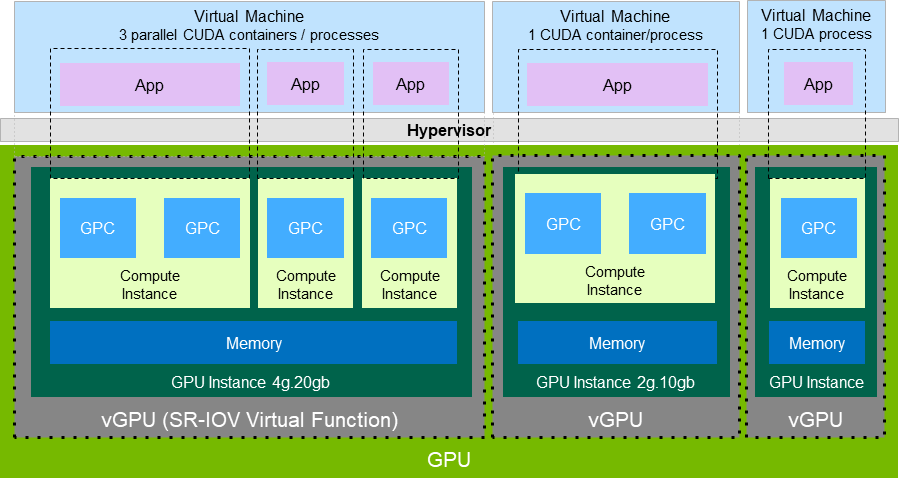
\includegraphics[width=\textwidth]{images/nvidia-vgpu-overview.png}
    \caption{GPU instances configured with Nvidia vGPU \cite{nvidia_vgpu_docs}}
    \label{fig:nvidia_vgpu_overview}
\end{figure}

\section{Pass-through model}
In the GPU pass-through model, a GPU is accessed directly by a single VM exclusively and permanently. This technique yields 96 to 100\% of native performance and high fidelity, but the acceleration provided by the GPU cannot be shared between multiple VMs. Hence, it has the lowest consolidation ratio and higher cost, as each graphics-accelerated VM requires an additional physical GPU. VMware's \textbf{vDGA} (Virtual Dedicated Graphics Acceleration) is one of the software technologies that implement fixed pass-through.

\section{Paravirtualized model}
In this software-based virtualization model, the hypervisor provides an API offering virtualization functions, and the guest OS in each VM then makes API calls that are forwarded to the host, and the host then executes these graphical commands from the guest OS using the host's GPU as a single user. This technique allows sharing GPU resources between multiple guests and a single host when the GPU \textbf{does not} support hardware-assisted virtualization. It is conceptually simple to implement. Hypervisors usually use shared memory between guest and host to maximize performance and minimize latency. VMWare's \textbf{vSGA} (Virtual Shared Graphics Acceleration) and QEMU/KVM's with \textbf{Virgil 3D} are the technologies that support this model.\\

\noindent VirGL is a virtual 3D GPU for use inside QEMU virtual machines that allows the guest OS to use the capabilities of the host GPU to accelerate 3D rendering. The rendering for the GPU is done in the host system as part of QEMU and is implemented purely on OpenGL, so one can get accelerated rendering on any sufficiently capable card/driver combination. Figure \ref{fig:virgl_stack} shows the VirGL stack. VirGL allows guest OS to simply feed it a series of OpenGL commands, and at the backend, these commands are fed into \textbf{virglrenderer}, which the physical GPU then renders on the host.\\

\begin{figure}[H]
    \centering
    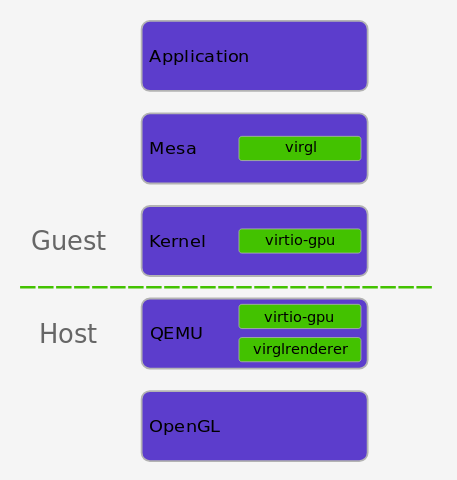
\includegraphics[width=0.5\textwidth]{images/virgl_stack.png}
    \caption{VirGL stack \cite{virgl_stack}}
    \label{fig:virgl_stack}
\end{figure}

\noindent virglrenderer is a backend for virtualized 3D graphics acceleration within the VMs. It supports the OpenGL API and translates OpenGL commands issued by the guest OS into instructions that the physical GPU in the host can understand and execute. So, the host does not know that a guest OS is using the GPU; for it, a VM utilizing the GPU is like any other OpenGL application running on the host.\\

\noindent \verb|virtio-gpu| and \verb|virtio-vga| are the paravirtualization frameworks QEMU provides to create a virtual GPU device and access it within a VM. The virtual GPU acts like a physical GPU attached to the VM. \verb|virtio-gpu| driver interacts with the virtual GPU and translates graphics commands from the guest OS into actions that the hypervisor understands and can pass on to the physical GPU on the host. This allows guest OS to render graphics directly onto the virtual display, minimizing latency and improving responsiveness.\\

\noindent \verb|virtio-vga|, similar to \verb|virtio-gpu|, emulates a standard VGA graphics adapter within the VM. This emulation provides basic graphics support, allowing the guest OS to display content on the screen using standard VGA modes and features. The difference between \verb|virtio-gpu| and \verb|virtio-vga| is that \verb|virtio-vga| provides a simpler and more basic graphics solution than \verb|virtio-gpu|. It ensures compatibility with legacy systems and software that rely on standard VGA graphics.

\subsection{What is virtio?}
In a paravirtualization environment, the guest OS is aware that it is running on a hypervisor and includes drivers that act as the front end. The hypervisor implements the back-end drivers for the particular device emulation. These front-end and back-end drivers are where \verb|virtio| comes in, providing a standardized interface for developing emulated device access to propagate code reuse and increase efficiency. \cite{virtio_ibm_article}\\

\begin{figure}[H]
    \centering
    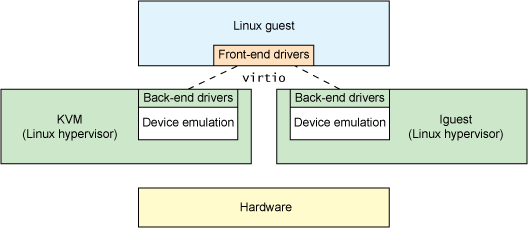
\includegraphics[width=0.7\textwidth]{images/virtio_stack.png}
    \caption{Driver abstractions with virtio \cite{virtio_ibm_article}}
    \label{fig:virtio_stack}
\end{figure}

\noindent When a VM boots up in QEMU, it communicates with the hypervisor to access resources like network interfaces or disk storage. QEMU provides \verb|virtio| drivers within the guest OS and helps the guest OS communicate with the hypervisor effectively. \verb|virtio| uses data structures called \textbf{virtqueues}, which act as a buffer to facilitate communication between the guest and the hypervisor.\\

\noindent In the VDI use case, the hypervisor needs to communicate with the GPU device. The \verb|virtio| drivers \verb|virtio-gpu| and \verb|virtio-vga| leverage the PCI (Peripheral Component Interconnect) bus architecture to communicate between the virtualized graphics devices and the hypervisor.\\

\noindent A good comparison between various Graphics Acceleration or GPU passthrough techniques is mentioned here: \url{https://cpaelzer.github.io/blogs/006-mediated-device-to-pass-parts-of-your-gpu-to-a-guest/}.\\

\noindent \textbf{Note}: While not as fast as the Hardware-assisted and Pass-through models, the major benefit of the Paravirtualized model is that it can be used without additional hardware and a proper input-output memory management unit (IOMMU) set up for device passthrough.

\section{QEMU/KVM based graphics acceleration}
We learned that \verb|virtio-gpu| and \verb|virtio-vga| are the \verb|virtio| drivers that provide a paravirtualized model for graphics acceleration. Graphics for QEMU/KVM comes with two important options, they are:

\begin{itemize}
    \item \verb|virtio-vga[-BACKEND]|: It is a basic version of the \verb|virtio-vga| device with optional backend support from virglrenderer.
    \item \verb|virtio-gpu[-BACKEND][-INTERFACE]|: This version also includes an additional option for an interface that can be VGA or non-VGA.
\end{itemize}

\noindent \textbf{Backend}: It determines how graphics are handled inside the guest. QEMU offers a 2D \verb|virtio-gpu| and \verb|virtio-vga| backend, but it provides an additional option for using accelerated backends like virglrenderer (labelled \verb|gl|), meaning \verb|virtio-gpu-gl| or \verb|virtio-vga-gl|, which provides 3D acceleration to the VM and improves the performance manifold than the default 2D backend.\\

\noindent \textbf{Interface}: It defines how the device communicates with the guest. VGA variants use the PCI interface by default. Non-VGA variants use either the MMIO or PCI interface. For PCI, one can use \verb|-pci| suffix.\\

\noindent Hence, a guest can have the following device configurations, namely:
\begin{itemize}
    \item \verb|virtio-vga|
    \item \verb|virtio-vga-gl|
    \item \verb|virtio-gpu|
    \item \verb|virtio-gpu-pci|
    \item \verb|virtio-gpu-gl-pci|
\end{itemize}

\noindent To get a list of the available \textbf{Display} devices supported by QEMU/KVM, run the below command. You will see the list of devices as shown in Figure \ref{fig:qemu_device_help}.\\
\texttt{qemu-system-x86\_64 -device help | grep -A 25 Display}

\begin{figure}[H]
    \centering
    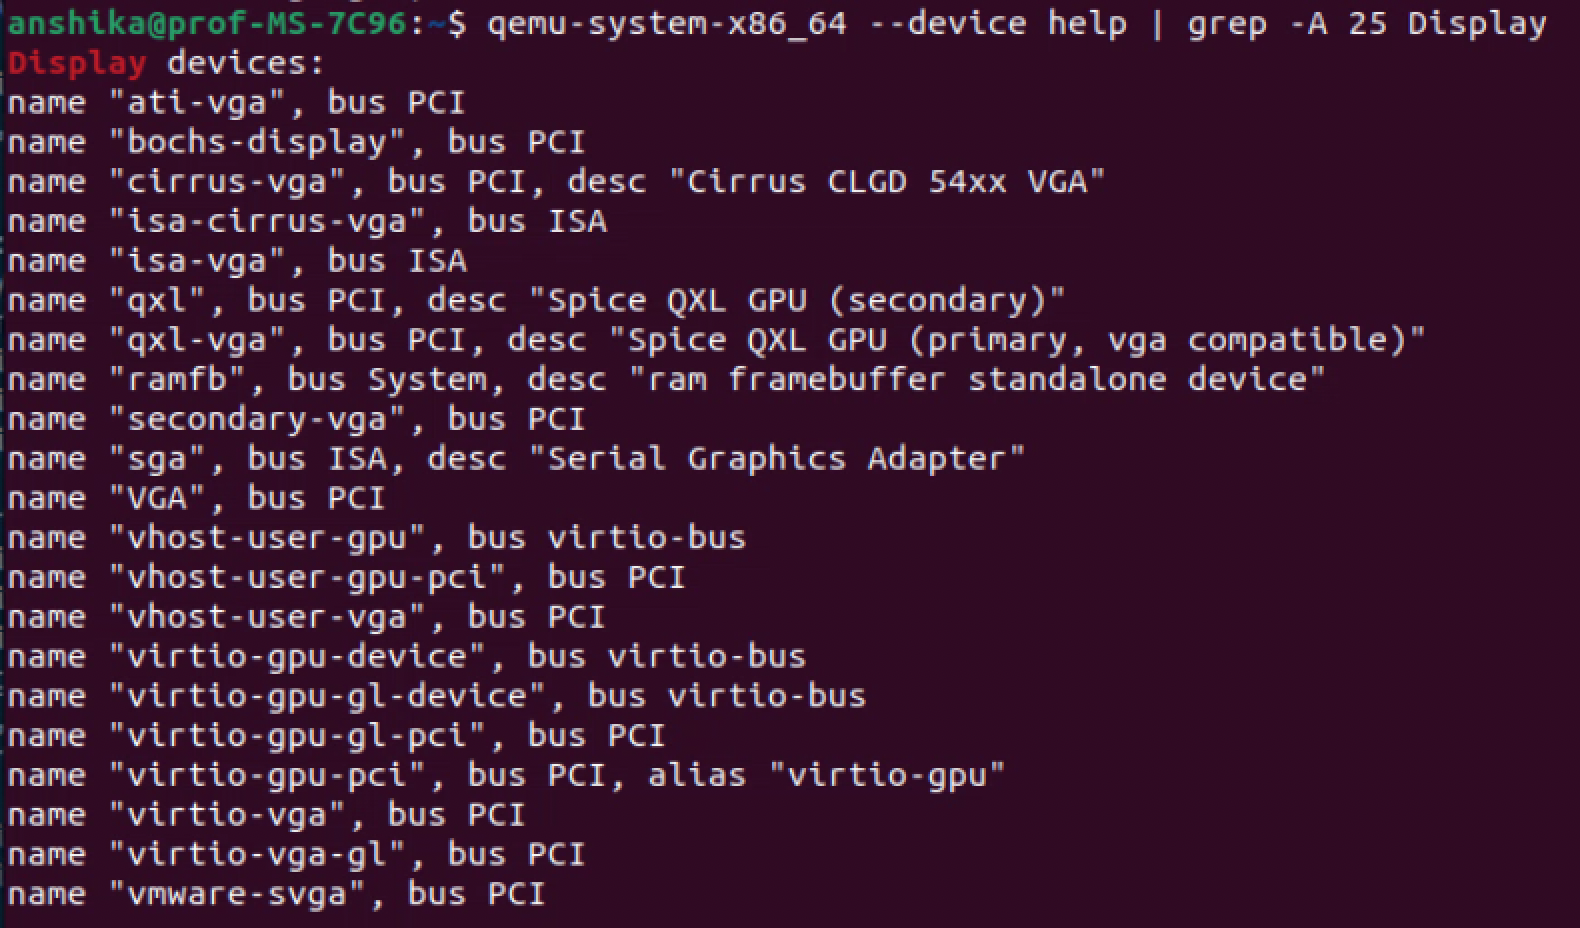
\includegraphics[width=0.8\textwidth]{images/device_help.png}
    \caption{Display devices supported by QEMU/KVM}
    \label{fig:qemu_device_help}
\end{figure}

\noindent The features of different display devices and their use cases are described quite well in this blog post: \url{https://www.kraxel.org/blog/2019/09/display-devices-in-qemu/}.

\begin{figure}[H]
    \centering
    \frame{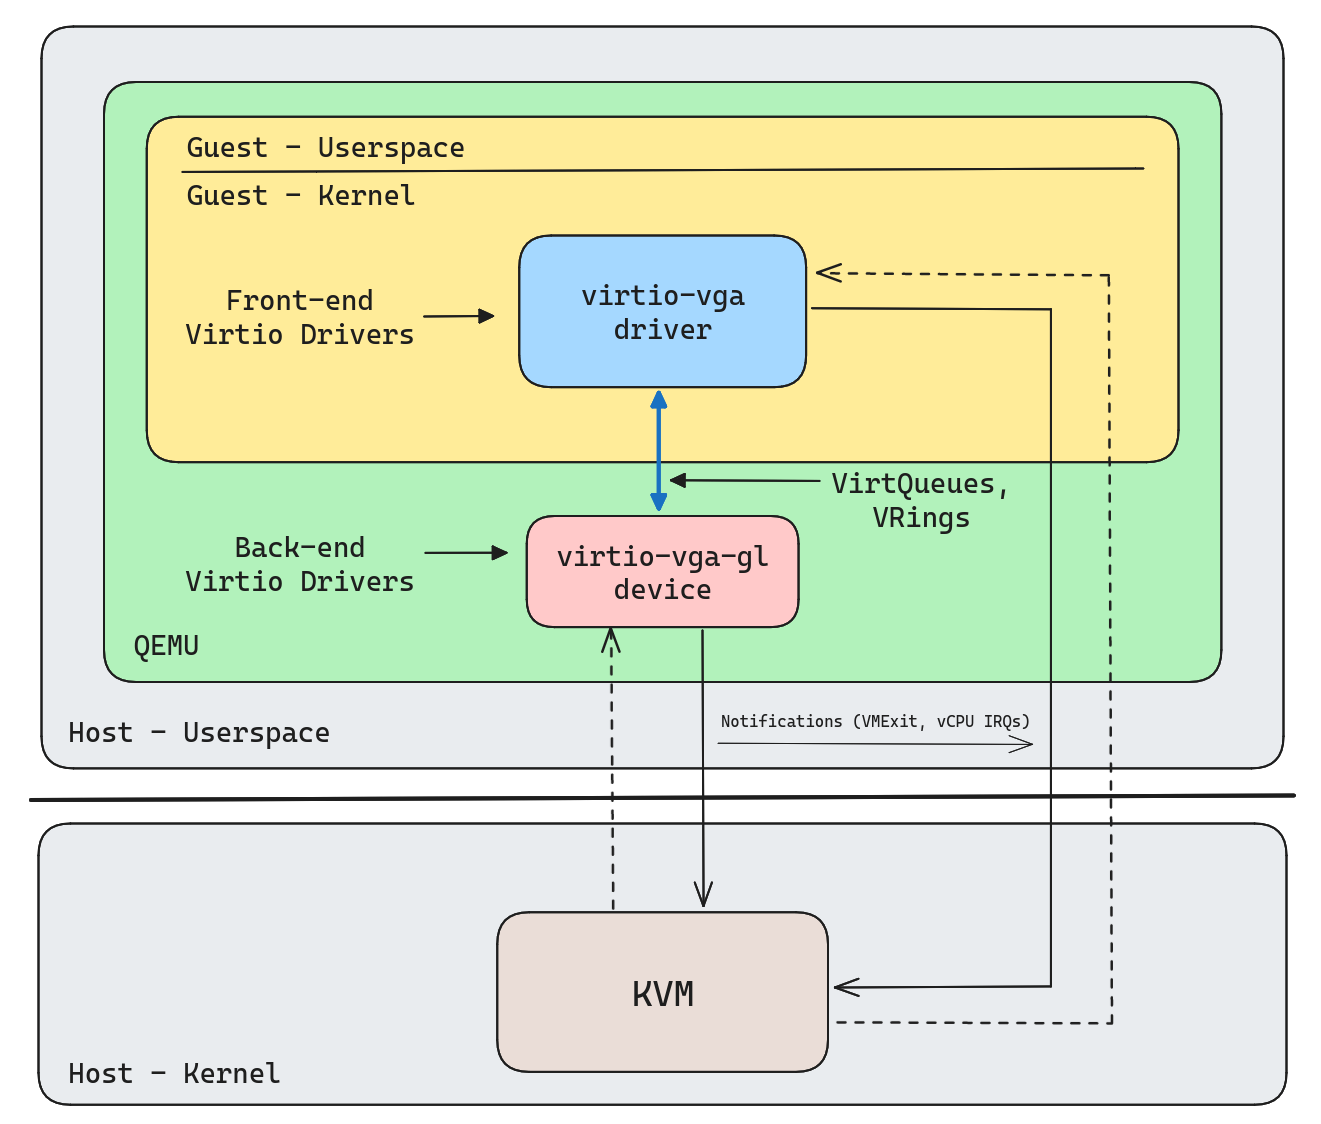
\includegraphics[width=0.8\textwidth]{images/virtio_vgpu_qemu_flow.png}}
    \caption{\texttt{virtio} architecture for GPU device}
    \label{fig:virtio_vgpu_qemu_flow}
\end{figure}

\noindent In the above figure \ref{fig:virtio_vgpu_qemu_flow}, we can see that the front-end \verb|virtio| drivers exist in the guest’s kernel, back-end \verb|virtio| devices exist in the hypervisor (QEMU), and communication between them is handled in the data plane via VirtQueues and VRings. We can also see notifications (e.g. VMExits, vCPU IRQs) from \verb|virtio| drivers and devices which are routed to KVM interruptions. The arrows indicate that the \verb|virtio-vga| driver and \verb|virtio-vga-gl| device interact with KVM for performing any privileged operation. KVM performs those operations on their behalf and replies with any necessary information.

\section{QEMU/KVM based display emulation}
\verb|-display| option determines which library QEMU will use to create the graphical interface inside the VM, \verb|sdl| or \verb|gtk|.

\begin{itemize}
    \item \verb|-display gtk|: It uses GTK (GIMP Toolkit) to create the graphical interface for displaying the guest's output. It is used in desktop applications that require a standard window with menus, buttons, sliders, etc. It provides a rich set of widgets for building complex user interfaces. It is heavier compared to other toolkits and libraries meant for simpler interfaces.
    \item \verb|-display sdl|: It uses SDL (Simple DirectMedia Layer) to create the graphical interface for displaying the guest's output. SDL is designed to provide low-level access to audio, keyboard, mouse, joystick, and graphics hardware via OpenGL and Direct3D. Often used in game development as it handles the graphics rendering, sound playback, and input management. Also used in applications that need direct control over these elements without the overhead of a full GUI toolkit. It is lightweight and flexible. Suitable for real-time applications such as games and multimedia software.
    \item \verb|-display [gtk/sdl],gl=on|: An optional \verb|gl=on| that enables 3D acceleration with GL context, use this option with either of \verb|virtio-gpu| and \verb|virtio-vga|.
\end{itemize}

\section{Graphics Acceleration in practice}
\noindent Launching a guest OS (of Linux Mint 21.3) using QEMU/KVM with the following options
\begin{itemize}
    \item \verb|-device virtio-vga-gl|
    \item \verb|-display sdl,gl=on|
\end{itemize}

\noindent creates a VM with the 3D acceleration enabled. To verify if that is the case, we can run the commands below in the guest OS.

\begin{enumerate}
    \item \verb|sudo lshw -C display|\\
            \begin{figure}[H]
                \centering
                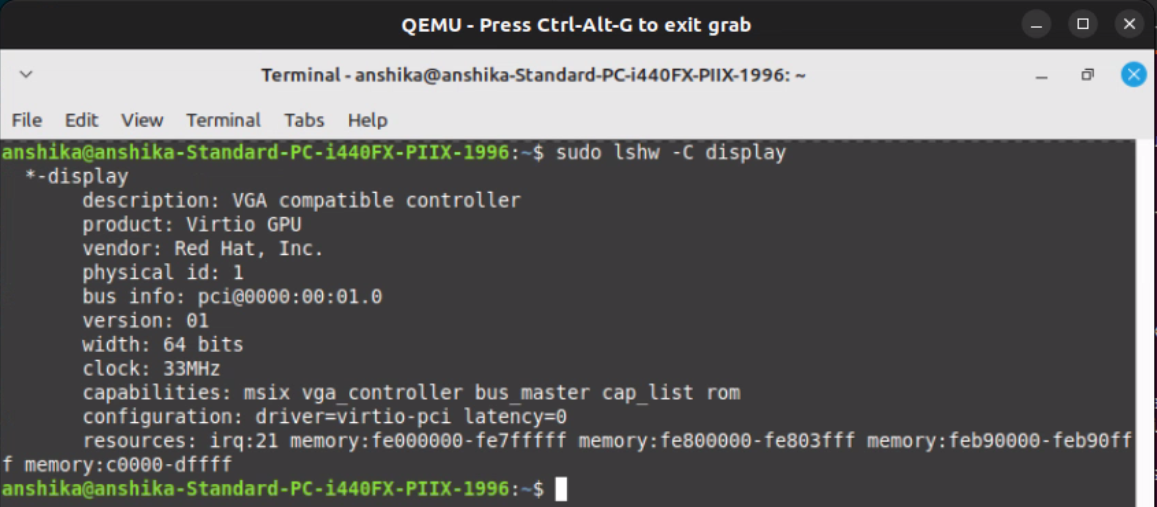
\includegraphics[width=0.8\textwidth]{images/virtio_gpu_lshw.png}
                \caption{lshw output with virtio-vga-gl inside a VM}
                \label{fig:lshw_hw_accel_vm}
            \end{figure}\\
            We can observe that the \verb|product| tag in the above image says \textbf{Virtio GPU}.
    \item \verb|glxinfo -B|\\
            \begin{figure}[H]
                \centering
                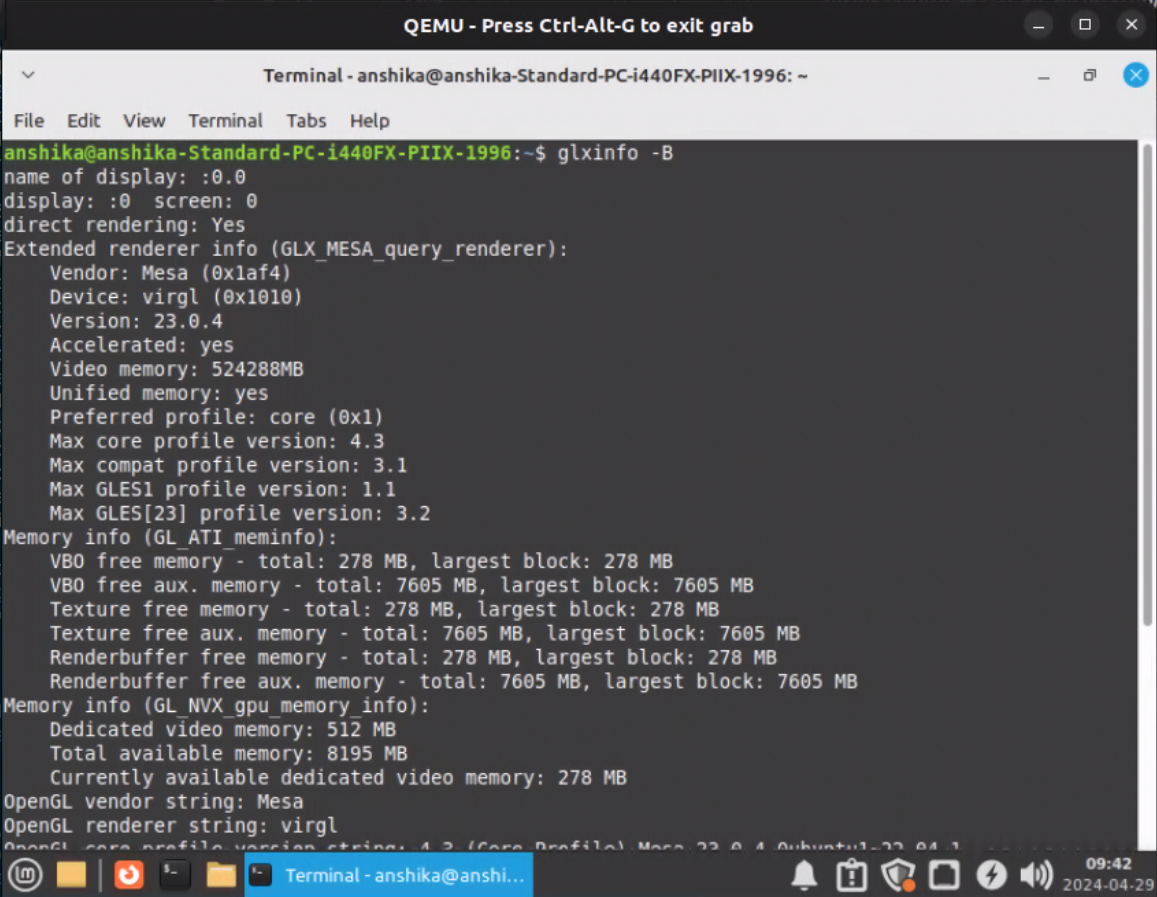
\includegraphics[width=0.8\textwidth]{images/virtio_gpu_glxinfo.png}
                \caption{glxinfo output with virtio-vga-gl inside a VM}
                \label{fig:glxinfo_hw_accel_vm}
            \end{figure}\\
            Here, the \verb|Device| is tagged as \textbf{virgl}, \verb|Accelerated| is \textbf{yes} and \verb|OpenGL renderer| \verb|string| also says \textbf{virgl}.
    \item \texttt{sudo dmesg | grep drm}\\
            \begin{figure}[H]
                \centering
                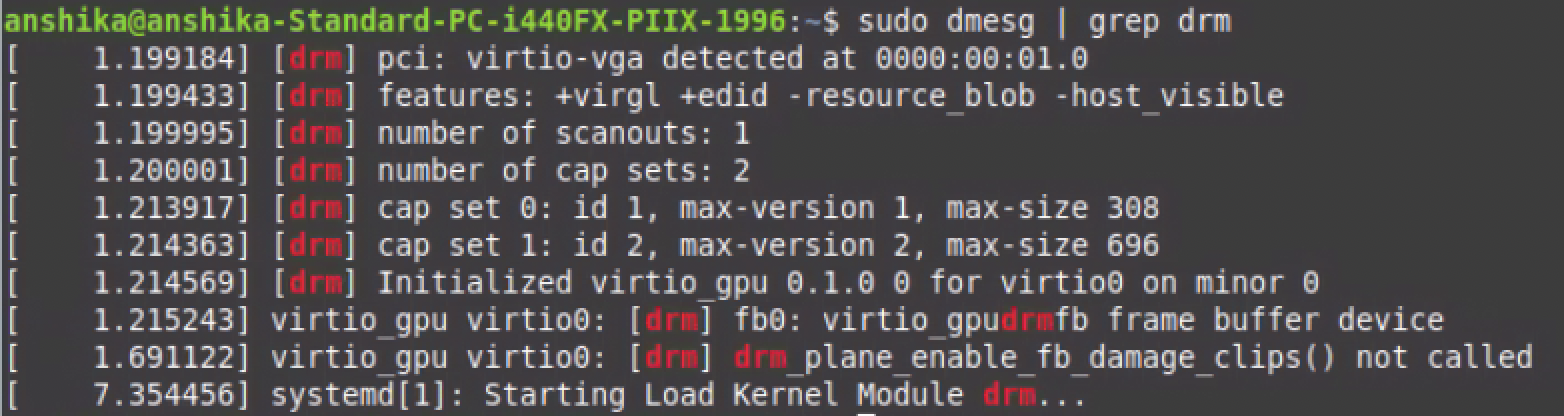
\includegraphics[width=0.8\textwidth]{images/dmesg.png}
                \caption{dmesg output with virtio-vga-gl inside a VM}
                \label{fig:dmesg_hw_accel_vm}
            \end{figure}\\
            The \verb|pci| device is mentioned as \textbf{virtio-vga}, which is a display device being used and under \verb|features|, \textbf{+} is shown as the prefix for \textbf{virgl}, that denotes the 3D hardware acceleration is on.
\end{enumerate}

\section{Performance Monitoring Tools}
Now that we know how to initiate a VM with hardware acceleration support, we should also look at some tools that can measure GPU performance and load when a task is scheduled. There are CLI and GUI tools. We will have a look at both one by one.

\subsection{CLI tools: htop, nvidia-smi, nvtop, radeontop, amdgpu\_top}
\begin{itemize}
    \item \textbf{htop}: It is a tool for monitoring all the processes running on the CPU. All the processes are listed here first, whether they utilize GPU or not. It also gives statistics on the amount of memory (RAM and swap) utilized. You can also select a process and send signals to it via this tool, for e.g. SIGKILL or SIGTERM. It can be installed via the command: \verb|sudo apt-get install htop|
    \item \textbf{nvidia-smi}: It is a utility provided by Nvidia for GPU utilization monitoring. However, its drawback is that it doesn't show process-wise break-up. Since it just shows a snapshot of the utilization, you can use \texttt{watch -n 1 nvidia-smi} to see real-time utilization. \texttt{nvidia-smi pmon} helps you see the process-wise encoder-decoder utilization. This tool is installed by default with the Nvidia drivers. % add link or in appendix on how to install nvidia drivers?
    \item \textbf{nvtop}: \href{https://github.com/Syllo/nvtop}{nvtop} tool is designed for monitoring the utilization of the GPUs from vendors like Intel, Nvidia, AMD, etc. It shows process-wise GPU utilization unlike \texttt{nvidia-smi}, and you do not have to add it to the watch specifically. One can install from apt: \verb|sudo apt-get install nvtop|
    \item \textbf{radeontop}: This is the same as nvtop, but specifically for AMD GPUs. It is available to install via apt: \verb|sudo apt-get install radeontop|
    \item \textbf{amdgpu\_top}: Another tool to display AMD GPU utilization. It also displays process-wise utilization like nvtop and information gathered from performance counters, sensors and drivers. It displays this information in GUI, TUI and JSON format, making it easier to parse the required values. One can download and install the latest deb package from the GitHub releases page: \url{https://github.com/Umio-Yasuno/amdgpu_top/releases}.
\end{itemize}

\subsection{GUI tool: Nsight-Systems}
It is a profiling tool provided by Nvidia for its GPUs. It gives a detailed breakdown of the resource utilization, including the function calls, system calls, ioctl calls, threads summary, and CPU utilization. However, this tool can collect GPU traces only for the recently manufactured GPUs. It supports GPU architectures Pascal or newer. \cite{nsight_sys_gpu_support} \\

\noindent Following snapshots depict the profiling done for the available Nvidia GPU GTX9701 (from Maxwell architecture \cite{gpu_gtx9701}) for the video encoding task using ffmpeg.\\

\begin{figure}[h]
    \centering
    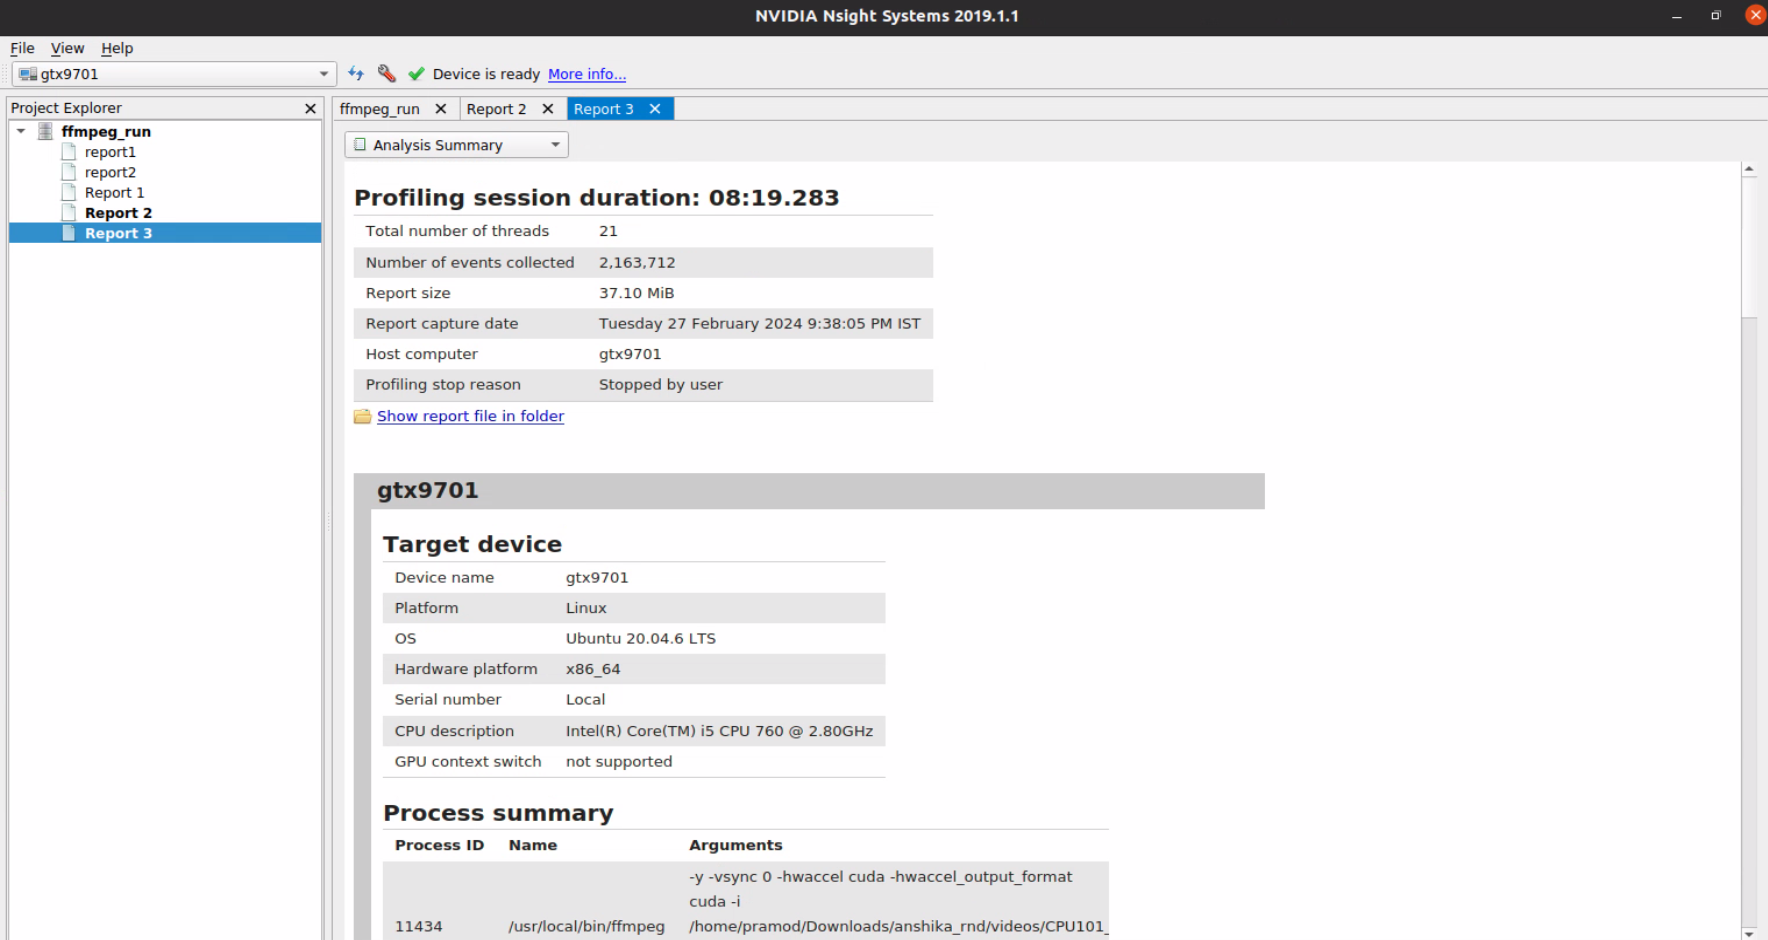
\includegraphics[width=0.85\textwidth]{images/nsight1.png}
    \caption{Adding target device (GPU) and task to profile}
    \label{fig:add_target_dev_nsight}
\end{figure}

\noindent Since we cannot collect GPU traces (as the GTX9701 is not supported, as it does not belong to Pascal or newer architectures), certain threads, like encode and decode, for the ffmpeg video encoding task, consume the CPU more than other threads. This is evident from the values observed in the Thread summary of Figure \ref{fig:thread_summ_nsight}.\\

\noindent The detailed profiling summary is shown in Figure \ref{fig:detailed_summ_nsight}. We can see that the function calls are made from the APIs by the respective encoding and decoding threads.

\begin{figure}[H]
    \centering
    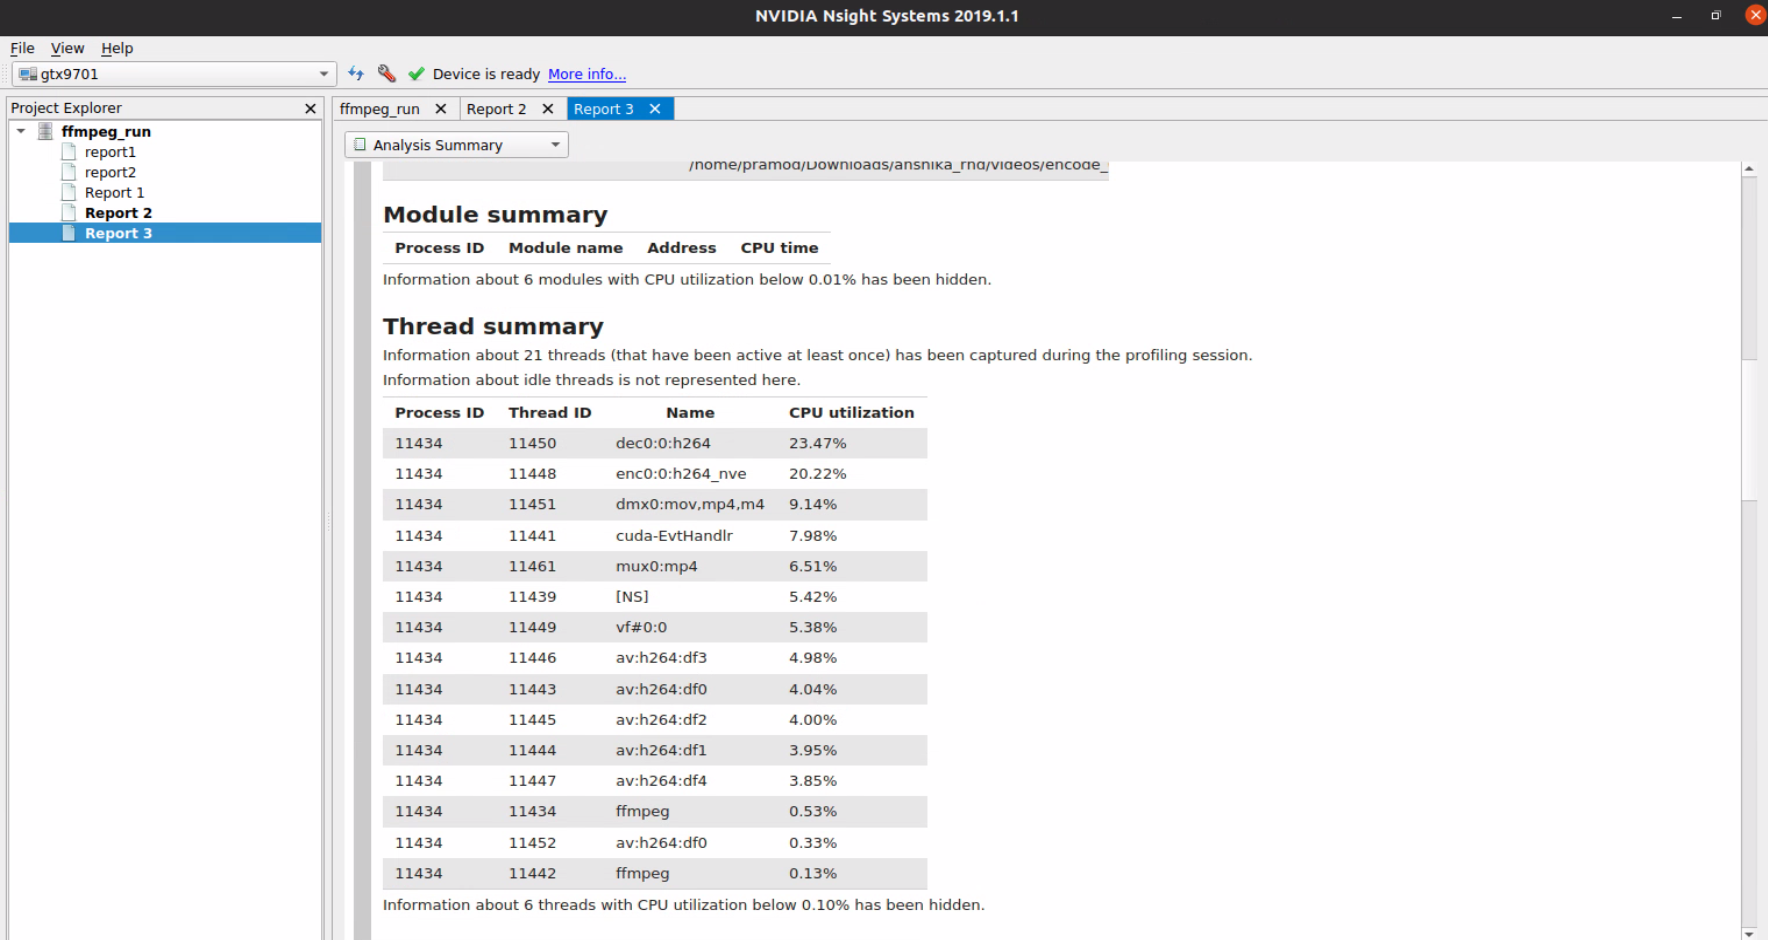
\includegraphics[width=0.85\textwidth]{images/nsight2.png}
    \caption{Thread summary of the video encoding task}
    \label{fig:thread_summ_nsight}
\end{figure}

\begin{figure}[H]
    \centering
    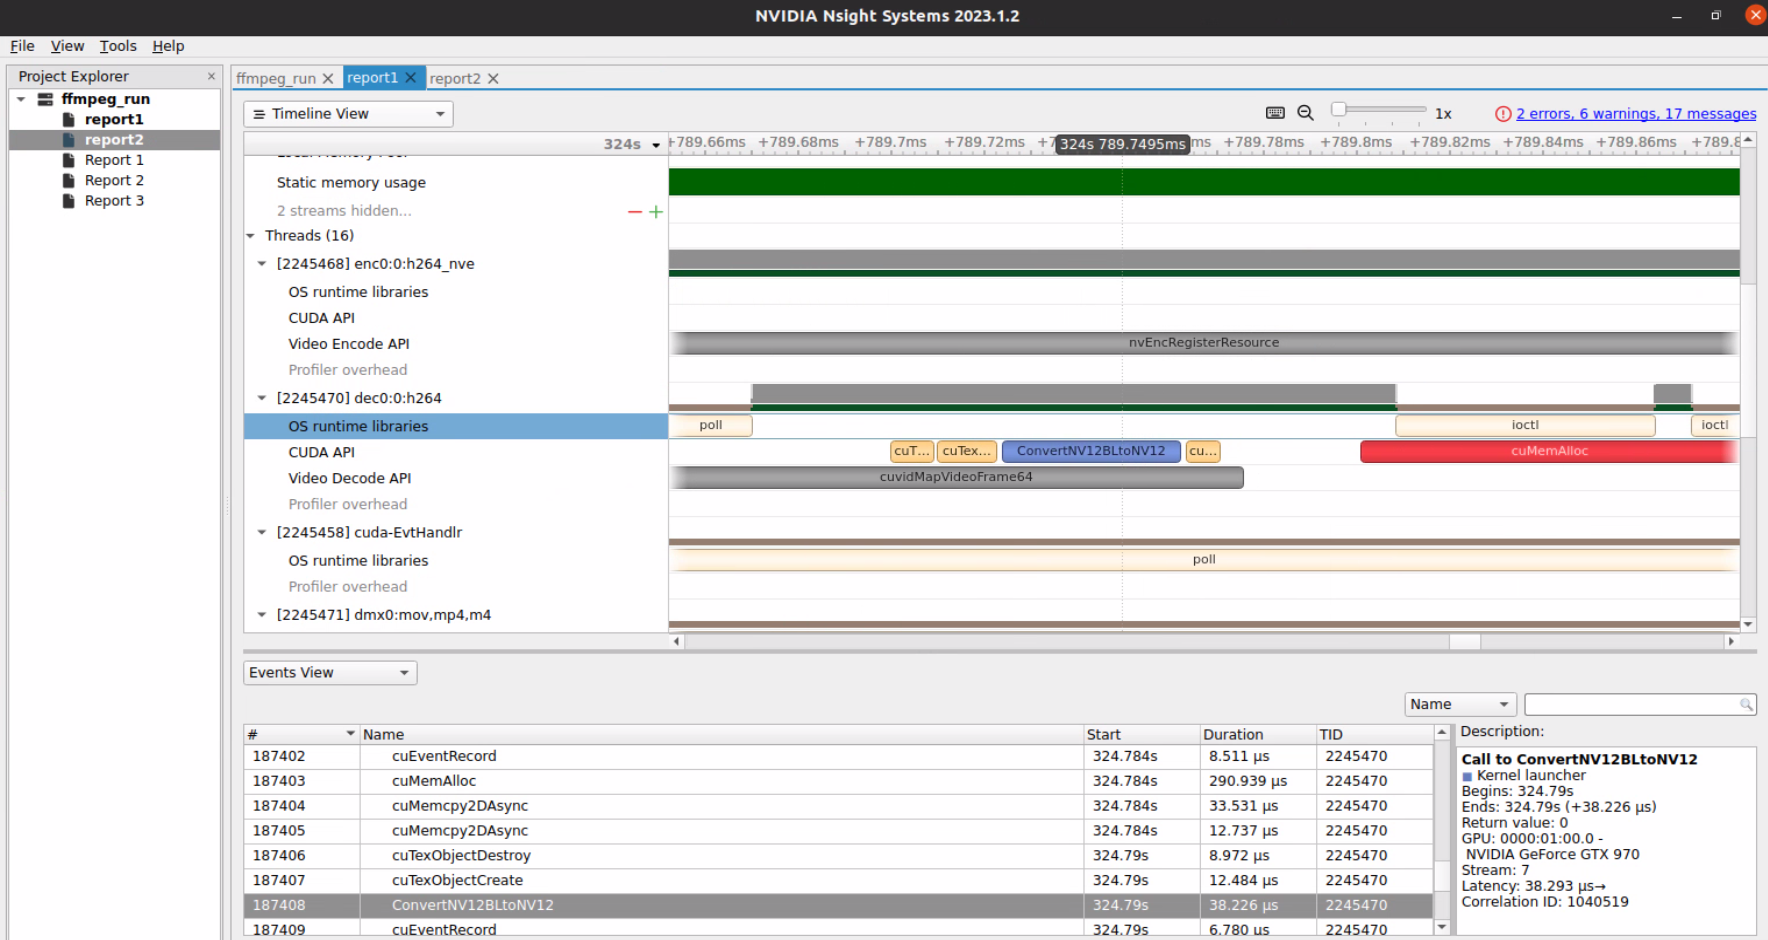
\includegraphics[width=0.85\textwidth]{images/nsight3.png}
    \caption{Detailed Summary of the video encoding task}
    \label{fig:detailed_summ_nsight}
\end{figure}

\noindent \textbf{System requirements for using Nsight-Systems GPU profiling}: As mentioned before, Pascal or newer GPUs are supported. To check if Nsight-Systems supports your GPU, run the command: \texttt{nsys profile --gpu-metrics-device=help}. The figure below shows the output of this command if the GPU is not supported.

\begin{figure}[H]
    \centering
    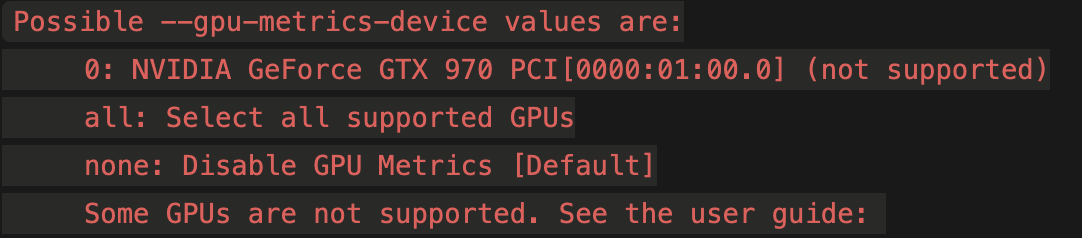
\includegraphics[width=\textwidth]{images/nsys_check.png}
    \caption{Check for GPU support by Nsight-Systems}
    \label{fig:nsys_check}
\end{figure}

\noindent Since we did not have a compatible Nvidia GPU that could be profiled using Nsight-Systems, our conclusions and performance characterisation are based on GPU utilization in the \verb|amdgpu_top|.

\section{Performance Evaluation of Graphics Acceleration} \label{dry_run_tests}
A couple of OpenGL programs are available that have been accepted as the \textbf{benchmark} by the community. One of these is \textbf{glmark2} available with \textbf{phoronix-test-suite}. \verb|glmark2| runs for a specific display resolution and provides a score at the end. The higher the score, the better the graphics acceleration.\\

\noindent Follow the steps below to install and run the benchmark from the test suite.

\begin{itemize}
    \item Make sure the virtualization software QEMU/KVM is installed.
    \begin{itemize}
        \item Follow this link for the steps: \url{https://help.ubuntu.com/community/KVM/Installation}.
        \item First, check whether the CPU supports hardware virtualization by installing the \verb|cpu-checker| package from apt (\verb|sudo apt install -y cpu-checker|) and running the command \verb|kvm-ok|.
        \item If the KVM virtualization is enabled, the command output should say: "KVM acceleration can be used".
    \end{itemize}
    \item Install mesa and glmark2\\
            \verb|sudo apt install mesa-utils glmark2|
    \item Install Phoronix test suite\\
            \verb|sudo apt install gdebi-core|\\
            Download the latest version \textbf{deb} package for the test suite from the GitHub releases page: \url{https://github.com/phoronix-test-suite/phoronix-test-suite/releases}.\\
            Then install the package\\
            \verb|sudo gdebi phoronix-test-*.deb|
    \item Run the test\\
            \verb|phoronix-test-suite benchmark glmark2|
\end{itemize}

\noindent With the host OS of Ubuntu 22.04 LTS, we first run the benchmark on the host (with the support of hardware acceleration) to form a baseline before proceeding with the VM-based tests. For consistency between the host and VM, we limit the test to the display resolution of \verb|800 x 600|.\\

\noindent Then we create the VM with and without the support of hardware acceleration and run the benchmark for both cases. Table \ref{tab:glmark2_tests_host_guest} highlights the benchmark scores for each test. The physical GPU available at the host is AMD Radeon Graphics (integrated with AMD Reyzen 5700G) with VRAM of 512 MB.\\

\noindent As expected, the host's benchmark score will be the largest as it has direct access to the GPU, while the VM has a virtual GPU available to work with. Also, the score of the test with the support of hardware acceleration is indeed larger than the one without it. This means that the physical GPU is being utilized to the required potential inside a VM.

\begin{table}[H]
\caption{glmark2 benchmark score for tests on host and guest}
    \label{tab:glmark2_tests_host_guest}
    \centering
    \begin{tabular}{|p{5cm}|c|c|p{4.5cm}|}
        \hline
        Test & VM count & Benchmark score & Comments \\ \hline
        Baseline for VM & 0 & 5602 & benchmark ran on host \\ \hline
        VM with no hardware acceleration & 1 & 469 & benchmark ran in guest \\ \hline
        VM with hardware acceleration & 1 & 3003 & benchmark ran in guest \\ \hline
    \end{tabular}
\end{table}

\noindent To know more about how the VM is set using the QEMU/KVM command line utility and the hardware acceleration performance with an increasing number of VMs w.r.t. the cost (i.e. GPU power and temperature), follow the next chapter.

% Chapter 4
\chapter{Analysis and Results}
This section describes the detailed working setup of a VM with the hardware acceleration support from QEMU/KVM. It also outlines the analysis of hardware acceleration support by running benchmark tests and evaluating based on certain metrics.

\section{Setting up a hardware-accelerated VM}
\noindent A default \verb|virt-manager| comes with Linux supporting the QEMU hypervisor, a GUI tool to set up a VM with a few of the features we listed in the previous section. However, this tool is not developed and maintained as frequently as the \verb|qemu| command line utility. Hence, we must manually craft a QEMU/KVM command to set up the VM with the required features.\\

\noindent But first, we need a raw disk image of an OS we want to run inside the VM. So, in the \verb|virt-manager|, we set up a VM with an ISO image by navigating to \texttt{File} > \texttt{Add New Machine} and add the ISO image of the OS of our choice and name the VM, let's say \verb|vm1|.\\

\noindent We used the \textbf{Linux Mint 21.3} OS because it is minimalistic and uses the desktop manager as Xfce. Other OSes like Ubuntu take up a lot of RAM just by running a single VM image, and hence, running multiple VMs with Ubuntu OS on a machine with 16 GB RAM seems a far-fetched idea. Download the Xfce edition of Linux Mint 21.3 from \href{https://www.linuxmint.com/edition.php?id=313}{this link}. Choose one of the mirrors to download it.\\

\noindent Once the OS is installed inside the VM, the raw disk image path of \verb|vm1.raw| is noted. This raw image is then converted into the format qemu requires using the command:

\noindent \verb|sudo qemu-img convert /var/lib/libvirt/images/vm1.qcow2 <path-to-vm1.raw>|

\noindent and we now use this image, \verb|vm1.qcow2|, to launch the VM using the \verb|qemu| command line.\\

%check-- form virt-manager once more
\noindent Following is the script we use to launch a VM with hardware acceleration support and network support from the default bridge network (\verb|virbr0|) created by QEMU-KVM.\\

\noindent An important note is that the \verb|virtio-gpu| with \verb|virgl| works only with QEMU version 6.2 and above. The QEMU version that you have installed depends on the Linux distro version. So, if you are using Ubuntu 20.04 and QEMU 4.2 has been installed, you need to upgrade your Ubuntu to 22.04 and reinstall the QEMU.\\

\newpage

\begin{mdframed}[backgroundcolor=cyan!20]
    \begin{lstlisting}[language=bash]
sudo qemu-system-x86_64 -boot c \
      -enable-kvm \
      -smp 3 \
      -device virtio-vga-gl,xres=800,yres=600 \
      -display sdl,gl=on \
      -cpu host \
      -m 8G \
      -vnc 0.0.0.0:1 \
      -drive file=/var/lib/libvirt/images/vm1.qcow2,
      if=virtio,aio=native,cache.direct=on,cache=writeback \
      -object rng-random,id=rng0,filename=/dev/urandom \
      -device virtio-rng-pci,rng=rng0 \
      -device virtio-keyboard-pci \
      -device virtio-mouse-pci \
      -serial none \
      -parallel none \
      -device virtio-tablet-pci \
      -device virtio-balloon \
      -device virtio-net-pci,netdev=bridge0 \
      -netdev bridge,id=bridge0,br=virbr0 \
      -machine q35,vmport=off \
      -boot menu=on \
      -daemonize
    \end{lstlisting}
\end{mdframed}

% \vspace{10pt}
% \subsection{QEMU Networking} \label{qemu_nw_section}
% need to write here

\section{Script dissection}
\begin{itemize}
    \item \texttt{qemu-system-x86\_64}: Binary for the command utility provided by QEMU-KVM
    \item \texttt{-boot c}: This option specifies boot order drives as a string of drive letters; \texttt{c} stands for hard disk boot.
    \item \texttt{-enable-kvm}: To enable KVM full virtualization support.
    \item \texttt{-smp 3}: To simulate an SMP (Symmetric multiprocessing or Shared-memory multiprocessing) system with 3 CPUs.
    \item \texttt{-device virtio-vga-gl,xres=800,yres=600}: Enable the backend device \verb|virtio-gpu| with hardware acceleration support (\verb|-gl|) and the display resolution of 800 x 600.
    \item \texttt{-display sdl,gl=on}: Display the video via SDL and enable 3D hardware acceleration.
    \item \texttt{-cpu host}: Enable all features of the host CPU.
    \item \texttt{-m 8G}: Sets the guest startup RAM size to 8 GB.
    \item \texttt{-vnc 0.0.0.0:1}: Configures QEMU to listen on the VNC display and redirect the VGA display over the VNC session. TCP connections are allowed from any client (due to 0.0.0.0, else only from the host in case of 127.0.0.1) that can ping the VM and on the port 5900 + 1 = 5901.
    \item \texttt{-drive file=/var/lib/libvirt/images/vm1.qcow2, \newline if=virtio,aio=native,cache.direct=on,cache=writeback}: Defines a new drive with the guest disk image of \verb|vm1.qcow2| with \verb|virtio| interface and the writeback mode for accessing block data from the host cache. You can find your file name using the virt-manager GUI options. 
    %check -- exactly which option
    \item \texttt{-object rng-random,id=rng0,filename=/dev/urandom}: To create a random number generator (RNG) backend by obtaining the entropy from the file \verb|/dev/urandom| on the host and assign a unique ID of \verb|rng0| that will be used to reference this entropy backend from \verb|virtio-rng| device.
    \item \texttt{-device virtio-rng-pci,rng=rng0}: Create a RNG device with the entropy backend referred as \verb|rng0| object.
    \item \texttt{-device virtio-keyboard-pci}: Add a virtio device for the keyboard with PCI interface.
    \item \texttt{-device virtio-mouse-pci}: Add a virtio device for the mouse with PCI interface.
    \item \texttt{-serial none}: Disable all serial ports from host.
    \item \texttt{-parallel none}: Disable all parallel ports from host.
    \item \texttt{-device virtio-tablet-pci}: Add a virtio device for the tablet with a PCI interface.
    \item \texttt{-device virtio-balloon}: A virtio device that can reclaim memory from a guest it isn't using and also supports reporting of guest memory statistics.
    \item \texttt{-netdev bridge,id=bridge0,br=virbr0}: Connect a host TAP network interface to a host bridge device, i.e. \verb|virbr0| which is created by default while installing QEMU-KVM. Assign a unique ID of \verb|bridge0| that will be used to reference from \verb|virtio-net| device,
    \item \texttt{-device virtio-net-pci,netdev=bridge0}: Create a network device with the bridge referred as \verb|bridge0| object.
    \item \texttt{-machine q35,vmport=off}: Selects an emulated machine by name; here, q35 adds emulation of the ICH9 (Intel I/O Controller Hub 9) host chiplet. Also, disable the emulation of the VMWare IO port.
    \item \texttt{-boot menu=on}: Enable the interactive boot menu.
    \item \texttt{-daemonize}: Daemonize the QEMU process after initialization.
\end{itemize}

% \subsection{QEMU Installation}
% \subsection{Additional Reading}
% Following is the list of few terms that I came across while figuring out this setup but since they were not as relevant, I haven't touched upon them in this document. They can be read upon as per interest and for better understanding.
% \begin{itemize}
%     \item QXL
%     \item egl-headless server
%     \item rendernode
%     \item SPICE server
%     \item 
% \end{itemize}

\section{Analysis of Hardware Acceleration}
Continuing from the section \ref{dry_run_tests}, we perform a sequence of tests (we call it experiments hereafter) with \verb|glmark2| benchmark with more than one hardware-accelerated VM running in parallel. For an experiment, we perform 3 runs to have non-biased results. We then consider the average of the metric values as the final value for that experiment setup.

\subsubsection{Configuration of the system under test}
\begin{itemize}
    \item Host OS: Ubuntu 22.04 LTS
    \item Host RAM: 16 GB
    \item GPU Name: AMD Radeon Graphics (integrated with AMD Reyzen 5700G)
    \item GPU Cores: 8
    \item GPU VRAM: 512 MB
    \item Monitoring tool used: \verb|amdgpu_top|
\end{itemize}

\subsubsection{Metrics for the system under test}
The metrics to be considered for analysing hardware acceleration are listed below. Apart from the \verb|glmark2| benchmark score, the values of other metrics are noted for the complete duration of the experiment, and then the maximum and average values are determined. A Python script runs on the host alongside the experiments in VM(s) to monitor these metric values.

\begin{itemize}
    \item \verb|glmark2| Benchmark score: indicates the GPU performance at the end of the test run (a performance parameter)
    \item Max. and Avg. GPU utilization (in \%): indicates the utilization of Compute Units in the GPU during the test run (a performance parameter)
    \item Max. and Avg. VRAM utilization (in \%): indicates the utilization of VRAM (Video RAM) during the test run (a performance parameter)
    \item Max. and Avg. CPU utilization (in \%): indicates the utilization of the host CPU during the test run, or in other words, the CPU load for running a test (a performance parameter)
    \item Max. and Avg. GPU Temperature (in deg. Celsius): indicates how much cooling is required for the safe operation of GPU (a cost parameter)
    \item Max. and Avg. GPU Power (in Watts): indicates the amount of load on the GPU (a cost parameter)
\end{itemize}

\noindent A \href{https://docs.google.com/spreadsheets/d/1hZbSorDnwsLE9Sq_sm1WylsL8ZV26K7jDEhZbVOg9KE/edit?usp=sharing}{spreadsheet} with all the metric values for each run of the experiment is populated.\\

\noindent Below are the plots for the experiments we performed with an increasing number of parallel running VMs. \vspace{20pt}

\begin{figure}[H]
    \centering
    \frame{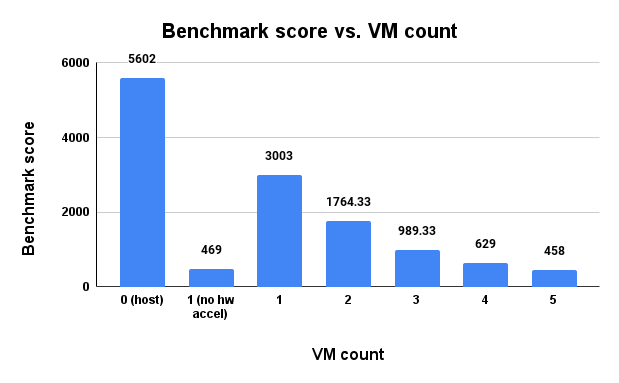
\includegraphics[width=0.7\textwidth]{images/plots/benchmark_score_vs_vm_count.png}}
    \caption{Benchmark score vs VM count}
    \label{fig:benchmark_score_vs_vm_count}
\end{figure}

\begin{figure}[H]
    \centering
    \frame{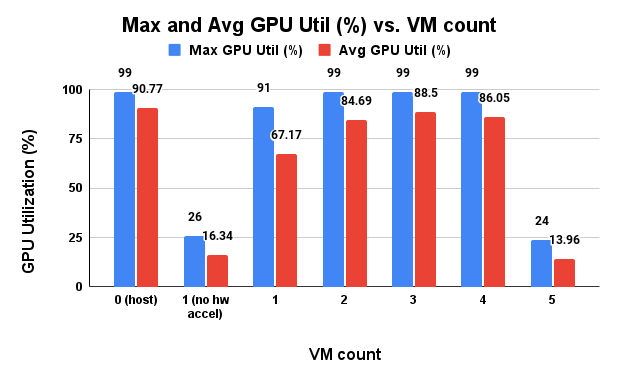
\includegraphics[width=0.7\textwidth]{images/plots/max_avg_gpu_util_vs_vm_count.png}}
    \caption{Max. and Avg. GPU Utilization (in \%) vs VM count}
    \label{fig:max_avg_gpu_util_vs_vm_count}
\end{figure}

\begin{figure}[H]
    \centering
    \frame{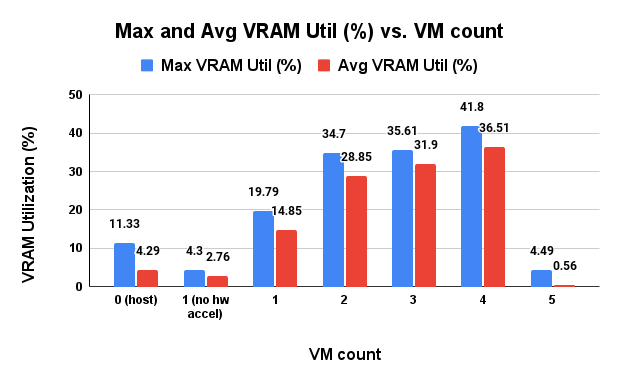
\includegraphics[width=0.7\textwidth]{images/plots/max_avg_vram_util_vs_vm_count.png}}
    \caption{Max. and Avg. VRAM Utilization (in \%) vs VM count}
    \label{fig:max_avg_vram_util_vs_vm_count}
\end{figure}

\begin{figure}[H]
    \centering
    \frame{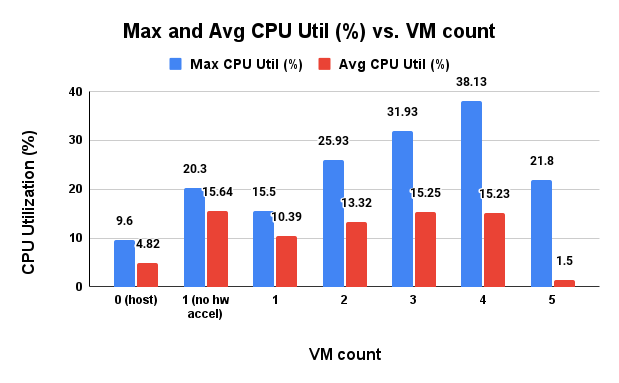
\includegraphics[width=0.7\textwidth]{images/plots/max_avg_cpu_util_vs_vm_count.png}}
    \caption{Max. and Avg. CPU Utilization (in \%) vs VM count}
    \label{fig:max_avg_cpu_util_vs_vm_count}
\end{figure}

\begin{figure}[H]
    \centering
    \frame{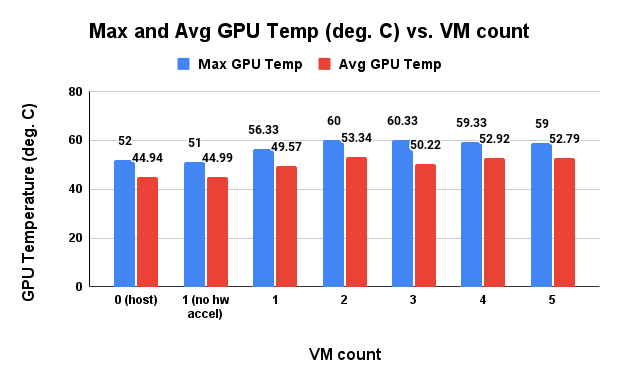
\includegraphics[width=0.7\textwidth]{images/plots/max_avg_gpu_temp_vs_vm_count.png}}
    \caption{Max. and Avg. GPU Temperature (in deg. Celsius) vs VM count}
    \label{fig:max_avg_gpu_temp_vs_vm_count}
\end{figure}

\begin{figure}[H]
    \centering
    \frame{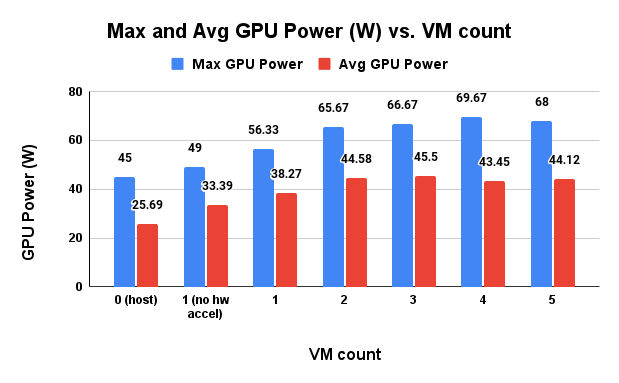
\includegraphics[width=0.7\textwidth]{images/plots/max_avg_gpu_power_vs_vm_count.png}}
    \caption{Max. and Avg. GPU Power (in Watts) vs VM count}
    \label{fig:max_avg_gpu_power_vs_vm_count}
\end{figure}

\section{Inference from the plots}
\begin{enumerate}
    \item With an increase in VM count, we see a decreasing trend in the Benchmark score (Figure \ref{fig:benchmark_score_vs_vm_count}) since the load on the virtual GPU and, hence, on the physical GPU increases. Beyond the VM count of 4, the Benchmark score is almost similar to the experiment of 1 VM with no support of hardware acceleration. Hence, we can say that for the given system under test, not more than 4 VMs can run in parallel with acceptable performance.
    \item In Figure \ref{fig:max_avg_gpu_util_vs_vm_count}, the maximum GPU utilization remains almost constant with increasing VM count. The average utilization has an increasing trend. For 5 VMs, it's highly probable that the frames are being dropped during the run. Also, the host RAM was close to full, so some swap memory was used. Hence, we can deduce that the tasks on the GPU were not running in parallel. Thus, we see very little max. and average GPU utilization for 5 VMs.
    \item The max. and average VRAM utilization (Figure \ref{fig:max_avg_vram_util_vs_vm_count}) also see an increasing trend with an increase in VM count as the load on the GPU increases. For 5 VMs, it's possible that the GPU is not rendering the benchmark properly on its Compute Units, hence the drop in VRAM utilization.
    \item For the CPU utilization (Figure \ref{fig:max_avg_cpu_util_vs_vm_count}), the average utilization is almost similar, and this should be the case, as the benchmark is utilizing the GPU and not CPU, unless in the case of 0 VMs (host) and 1 VM with no support of hardware acceleration. For the VM count of 5, the value seems to be corrupted. The max. utilization values have an increasing trend; the reason could be that some background processes utilized the CPU for a large fraction but in a small timeframe.
    \item The GPU temperature and power (Figures \ref{fig:max_avg_gpu_temp_vs_vm_count} and \ref{fig:max_avg_gpu_power_vs_vm_count}) do not show much variation w.r.t. change in VM count. This indicates that regardless of the load on the GPU, the current drawn was almost constant, hence the power consumption and temperature.
\end{enumerate}

\section{Analysis of GPU-accelerated VDI}
As described in Table \ref{tab:glmark2_tests_host_guest}, the same set of tests were run with and without the support of VDI, NoMachine in this case. Below Table \ref{tab:glmark2_tests_host_guest_vdi} highlights the Benchmark score for the same.

\subsection{Inference drawn}
\begin{itemize}
    \item It is evident from Table \ref{tab:glmark2_tests_host_guest_vdi} that the Benchmark scores will be less when the test is run from the NoMachine Client as compared to running it on the machine itself (host or VM).
    \item Also, the tests with VDI setup could not be carried with more than one VM since the VM is attached to a host bridge device, i.e. \verb|virbr0|. Hence, each VM created with this setup is allotted the same IP address accessible from the host machine, even though the display sessions are independent. Thus, the VMs are only accessible from within the host network.
\end{itemize}

\begin{table}[H]
\caption{glmark2 benchmark score for tests on host and guest (with and without NoMachine VDI)}
    \label{tab:glmark2_tests_host_guest_vdi}
    \centering
    \begin{tabular}{|p{3.5cm}|c|c|c|p{3.5cm}|}
        \hline
        Test & VM count & NoMachine & Benchmark score & Comments \\ \hline
        Baseline for VM & 0 & No & 5602 & benchmark ran on host \\ \hline
        Baseline for VDI & 0 & Yes & 5325 & benchmark ran on host from NoMachine \\ \hline
        VM with no hardware acceleration & 1 & No & 469 & benchmark ran in guest \\ \hline
        VM with no hardware acceleration & 1 & Yes & 314 & benchmark ran in guest from NoMachine \\ \hline
        VM with hardware acceleration & 1 & No & 3003 & benchmark ran in guest \\ \hline
        VM with hardware acceleration & 1 & Yes & 2027 & benchmark ran in guest from NoMachine \\ \hline
    \end{tabular}
\end{table}

% Chapter 5
\chapter{Conclusions and Future Scope}
%vnc, tap device, better performance characterisation method/metric maybe by using nsight systems

The current VDI setup with Graphics Acceleration is not fully functional for remote clients. One of the solutions is to set up a tap device in the host that can assign a unique public IP address to each VM being launched. This will make each VM accessible from outside the host network, just like a remote desktop connection. Although, the unpaid version of NoMachine does not allow more than one concurrent connection. With the paid version, we can access the VMs hosted on a server machine via VNC as well.\\

\noindent Nsight-Systems can profile the GPU more accurately and indicate the presence of bottlenecks, if any, or the mechanisms and configurations that can improve the GPU performance. This is possible, given that we have GPUs from Pascal or newer architecture to work with.\\

\noindent TurboVNC + VirtualGL setup can also be an alternative solution to the QEMU/KVM + NoMachine for the hardware-accelerated VDI setup. For better performance characterization, there needs to be a metric specific to VNC, as the TurboVNC paper \cite{turbovnc_report} uses for their performance improvement claim, like compression ratio.\\

\noindent There are ample resources available over the Internet for this setup and performance characterization, but one needs to understand the jargon to determine the path that can lead to a solution, provided we have the latest hardware available.

% \bibliographystyle{unsrt}
% \bibliographystyle{ieeetr}
% \bibliography{thesisTemplate}
\printbibliography

\end{document}

